\chapter{Теория вероятностей}

\section{test}
playground


\section {Условная вероятность. Независимость событий. Критерий независимости. Формула полной вероятности. Формула Байеса}

\begin{defn}
    Пусть задано вероятностное пространство $(\Omega, \mathcal{F}, \mathbb{P})$, ${A, B \in \mathcal{F}, \, \myprob{B} > 0}$. {\it Условная вероятность события $A$ при событии~$B$}:
    \begin{equation*}
        \myprob{A|B}=\cfrac{\myprob{AB}}{\myprob{B}}
    \end{equation*}
\end{defn}

\begin{thm*}
    Условная вероятность $\myprob{A|B}$~--- вероятность, заданная на $\mathcal{F}$.
\end{thm*}

\begin{proof}
    Проверим три аксиомы из определения вероятности.

\begin{enumerate}
    \item $\forall A \in \mathcal{F} \quad \myprob{A|B} \geqslant 0, \text{т.к.}~ \myprob{AB} \geqslant 0,~ \myprob{B} > 0$
    \item  $\myprob{\Omega|B} = \cfrac{\myprob{B \cap \Omega}}{\myprob{B}} = \cfrac{\myprob{B}}{\myprob{B}} = 1$
    \item Пусть дана некоторая последовательность событий $\it A_1, A_2, \ldots A_n, \ldots$; $A_i \cap A_j = \varnothing \: ({\it i \ne j})$. Тогда: 
    \begin{multline*}
        \mathbb{P}\left(\,\left. \bigcup\limits_{i=1}^\infty A_i \right| B\right)  = \cfrac{\mathbb{P}\left(\left(\bigcup\limits_{i=1}^\infty A_i\right) \cap B\right)}{\myprob{B}} = \cfrac{\mathbb{P}\left(\bigcup\limits_{i=1}^\infty\left(A_i \cap B\right)\right)}{\myprob{B}} = \\
        = \cfrac{\sum\limits_{i=1}^\infty \myprob{A_i \cap B}}{\myprob{B}}
        = \sum\limits_{i=1}^\infty \myprob{A_i | B}.
    \end{multline*}
\end{enumerate}
\end{proof}
\begin{rmrk}
    Некоторые свойства условной вероятности:
    \begin{enumerate}
        \item Если $A \cap B = \varnothing,$ то $\myprob {A | B} = 0.$ 
        \item Если $B \subset A$, то $\myprob{A|B} = 1.$ Например, $\myprob{B|B} = 1.$
    \end{enumerate}
\end{rmrk}

\subsubsection{Независимость событий}

\begin{defn}
    Пусть есть вероятностное пространство $(\Omega, \mathcal{F}, \mathbb{P})$. События $A_1, \ldots, A_n \in \mathcal{F}$ называются {\it независимыми в совокупности}, если $\forall k \in \overline{2, n}$ и $\forall i_{1}, \ldots, i_{k} \colon 1 \leqslant i_1 < i_2 < \ldots < i_k \leqslant n$ выполняется 
    \begin{equation*}
        \mathbb{P}\left(\bigcap\limits_{j=1}^k A_{i_j}\right) = \prod\limits_{j=1}^k \myprob{A_{i_j}}
    \end{equation*}

Иными словами, события независимы в совокупности, если вероятность одновременного наступления любого набора из этих событий равна произведению вероятностей событий, входящих в этот набор. В частности, при $n = 2$: события $A$ и $B$ независимы, если $\myprob{AB} = \myprob{A}\myprob{B}$.
\end{defn}

\begin{namedthm}[Свойства независимых событий]\leavevmode
    \begin{enumerate}
        \item Если $A = \varnothing$ или $\myprob{A} = 0$, то $\forall B \colon \myprob{B} > 0$ события $A$ и $B$ независимы.
        \item Пусть $A$ и $B$ независимы. Тогда события $\overline{A}$ и $B$, $A$ и $\overline{B}$, $\overline{A}$ и $\overline{B}$ также независимы. 
        \item Пусть $A \subset B$ и $\myprob{A} > 0, \, \myprob{B} < 1$. Тогда $A$ и $B$ зависимы. 
        \item Если события $A$ и $B$ независимы и $\myprob{B} > 0$, то $\myprob{A|B} = \myprob{A}$.
    \end{enumerate}
\end{namedthm}

\begin{proof}
\begin{enumerate} 
    \item Если $A = \varnothing$, то $AB = \varnothing \Rightarrow \myprob{AB} = 0.$ Но $ \myprob{A}\myprob{B} = 0 \cdot \myprob{B} = 0 \Rightarrow \myprob{AB} = \myprob{A} \myprob{B}$.
    
    Если же ${\myprob{A} = 0}$, то ${AB \subset A \Rightarrow \mathbb{P}(AB) \leqslant \myprob{A} = 0}$. В то же время ${0 = \myprob{AB} = 0 \cdot \myprob{B} = \myprob{A} \myprob{B}}$.

    \item Докажем независимость $\overline{A}$ и $B$, представив последнее в виде $B = AB \cup \overline{A}B$. Тогда
    \begin{multline*}
        \myprob{B} = \myprob{AB} + \myprob{\overline{A}B} = \myprob{A}\myprob{B} + \myprob{\overline{A}B} \Rightarrow \\
        \Rightarrow \myprob{\overline{A}B} = \myprob{B} - \myprob{A}\myprob{B} = \myprob{B} (1 - \myprob{A}) = \myprob{\overline{A}}\myprob{B}
    \end{multline*}
    Независимость $\overline{A}$ и $B$ доказана. Аналогично доказываются остальные утверждения.
    \item Предположим, что события независимы. Тогда $\myprob{AB} = \myprob{A}\myprob{B},$ но в силу вложенности $A \subset B$: $\myprob{AB} = \myprob{A}$, следовательно, $\myprob{B} = 1$, что противоречит условию.
    \item $\myprob{A | B} = \cfrac{\myprob{AB}}{\myprob{B}} = \cfrac{\myprob{A}\myprob{B}}{\myprob{B}} = \myprob{A}$
\end{enumerate}
\end{proof}

\begin{rmrk}
    В общем случае из попарной независимости событий $A_1, \ldots, A_n$ не следует их независимость в совокупности.
    \begin{exmp}
        Рассмотрим вероятностное пространство, в котором всего 4 различных элементарных исхода: $\Omega = \{\omega_1, \omega_2, \omega_3, \omega_4 \}$. Пусть $\mathcal{F}$~--- множество всех подмножеств $\Omega,~\myprob{\{\omega_i\}} = \cfrac{1}{4},~i = \overline{1,4}$.
        
        Рассмотрим три события 
        \begin{equation*}
            A_1 = \{\omega_1, \omega_4 \},~ 
            A_2 = \{\omega_2, \omega_4 \},~
            A_3 = \{\omega_3, \omega_4 \}
        \end{equation*}
        
        Их пересечения имеют вид:
        \begin{equation*}
            A_1A_2 = A_2A_3 = A_3A_1 = \{\omega_4 \},~
            A_1A_2A_3 = \{\omega_4 \}
        \end{equation*}
        
        Докажем, что события $A_1, A_2, A_3$ не являются независимыми в совокупности:
        \begin{gather*}
            \myprob{A_1} = \myprob{A_2} = \myprob{A_3} = \cfrac{1}{2}, \; \myprob{A_1A_2} = \myprob{A_2A_3} = \myprob{A_3A_1} = \cfrac{1}{4}, \\ \myprob{A_1A_2A_3} = \cfrac{1}{4} \neq \cfrac{1}{8} = \myprob{A_1}\myprob{A_2}\myprob{A_3}
        \end{gather*}
    \end{exmp}
\end{rmrk}

\begin{symb}
    \begin{equation*}
        A_{i}^{(\delta)} =
        \begin{cases}
            A_{i}, & \delta = 1; \\
            \overline{A_{i}}, & \delta = 0.
        \end{cases}
    \end{equation*}
\end{symb}

\begin{namedthm}[Критерий независимости]
    События $A_1, \ldots, A_n$ независимы в совокупности $\Leftrightarrow \forall ~ \delta_1, \delta_2, \ldots \delta_n \in \{0, 1\}$ выполнено равенство
    \begin{equation*}
        \mathbb{P}\left( \bigcap_{i=1}^{n} A_{i}^{\left( \delta_{i} \right)} \right)
        = \prod_{i=1}^{n}\mathbb{P}\left( A_{i}^{\left(\delta_{i}\right)} \right)
    \end{equation*}
\end{namedthm}

\begin{namedthm}[Формула полной вероятности]
    Пусть даны события $A, B_1, \ldots, B_n, \ldots$; $\myprob{B_i} > 0, $ причём $B_i B_j = \varnothing~(i \neq j)$ и $\bigcup\limits_{i=1}^{\infty}B_i \supset A~$ (например, $\bigcup\limits_{i=1}^{\infty}B_i = \Omega$). Тогда справедлива формула:
\begin{equation*}
    \mathbb{P}(A)=\sum\limits_{i=1}^{\infty} \mathbb{P}\left(B_{i}\right) \cdot \mathbb{P}\left(A | B_{i}\right)
\end{equation*}
\end{namedthm}

\begin{proof}
    Достаточно заметить, что при вышеперечисленных условиях $A = \bigcup\limits_{i=1}^{\infty}(AB_i),$ и $AB_i \cap AB_j = \varnothing ~(i \neq j).$ Тогда, учитывая $\myprob{B_i} > 0$, получаем
    \begin{equation*}
        \mathbb{P}(A)=\sum\limits_{i=1}^{\infty} \mathbb{P}\left(A B_{i}\right)=\sum\limits_{i=1}^{\infty} \mathbb{P}\left(B_{i}\right) \frac{\mathbb{P}\left(A B_{i}\right)}{\mathbb{P}\left(B_{i}\right)}=\sum\limits_{i=1}^{\infty} \mathbb{P}\left(B_{i}\right) \cdot \mathbb{P}\left(A | B_{i}\right)
    \end{equation*}
\end{proof}

\begin{namedthm}[Формулы Байеса]
    Пусть даны события $A, H_1, \ldots, H_n, \ldots$; ${\myprob{A} > 0}$, ${\myprob{H_i} > 0}$, причём $H_i H_j = \varnothing ~(i \neq j)$ и $\bigcup\limits_{i=1}^\infty H_i \supset A$ (например, $\bigcup\limits_{i=1}^{\infty}H_i = \Omega$). Тогда справедливы {\it формулы Байеса}:
    \begin{equation*}
        \mathbb{P}\left(H_{i} | A\right)= \frac{\mathbb{P}\left(H_{i}\right) \cdot \mathbb{P}\left(A | H_{i}\right)}{\sum\limits_{j=1}^{\infty} \mathbb{P}\left(H_{j}\right) \cdot \mathbb{P}\left(A | H_{j}\right)}, \quad i = \overline{1,n}
    \end{equation*}
\end{namedthm}
\begin{proof}
    Согласно формуле полной вероятности, в знаменателе дроби стоит вероятность $A$. Тогда
    \begin{equation*}
        \frac{\mathbb{P}\left(H_{i}\right) \cdot \mathbb{P}\left(A | H_{i}\right)}{\mathbb{P}(A)}=\frac{\mathbb{P}\left(H_{i}\right) \cdot \mathbb{P}\left(A H_{i}\right)}{\mathbb{P}(A) \cdot \mathbb{P}\left(H_{i}\right)}=\frac{\mathbb{P}\left(A H_{i}\right)}{\mathbb{P}(A)}=\mathbb{P}\left(H_{i} | A\right) 
    \end{equation*}
\end{proof}

Вероятности $P(H_i)$, вычисленные заранее, до проведения эксперимента, называют {\it априорными вероятностями} (a’priori~--- «до опыта»). Условные вероятности $\myprob{H_i | A}$ называют {\it апостериорными вероятностями} (a’posteriori~--- «после опыта»). Формула Байеса позволяет переоценить заранее известные вероятности после того, как получено знание о результате эксперимента.

\begin{exmp}
    Тест на рак имеет надёжность $99\%$ (т.е. вероятность как положительной, так и отрицательной ошибки равна $0,01$), рак появляется у $1\%$ населения. Какова вероятность того, что человек болен раком, если у него позитивный результат теста?
    
    Составим таблицу для вероятностей всех возможных событий:
    \begin{center}
    \begin{tabular}{|c|c|c|}
    \hline \multirow{2}{*} {Результат теста} & \multicolumn{2}{|c|} {Пациент реально болен} \\
    \cline {2-3} & Да & Нет \\
    \hline Положительный & $0,99 \cdot 0,01$ & $0,01 \cdot 0,99$ \\
    \hline Отрицательный & $0,01 \cdot 0,01$ & $0,99 \cdot 0,99$ \\
    \hline
    \end{tabular}
    \end{center}
    
    Введём следующие обозначения для событий: $H_{+} = \{\text{пациент болен}\}$, $H_{-} = \{\text{пациент здоров}\}$, $R_{+} = \{\text{положительный результат теста}\}$, $R_{-} = \{\text{отрицательный результат теста}\}$. Найдём вероятность события $H_{+}$ при условии $R_{+}$ по формуле Байеса:
    \begin{multline*}
        \mathbb{P}(H_{+}|R_{+}) = \cfrac{\mathbb{P}(H_{+})\mathbb{P}(R_{+}|H_{+})}{\mathbb{P}(H_{+})\mathbb{P}(R_{+}|H_{+}) + \mathbb{P}(H_{-})\mathbb{P}(R_{+}|H_{-})} = \\
        = \cfrac{0,99 \cdot 0,01}{(0,99 \cdot 0,01) + (0,01 \cdot 0,99)} = 0,5
    \end{multline*}
    
    Иными словами, вероятность того, что пациент болен, равна отношению вероятности правильного положительного результата теста к вероятности любого положительного результата.
    
    Рассмотрим более общий случай. Пусть $q$~--- вероятность неправильного результата теста, $p$~--- вероятность заболеть раком, тогда
    \begin{equation*}
        \mathbb{P}(H_{+}|R_{+}) 
        = \cfrac{(1-q) p}{(1-q) p+q(1-p)} 
        = \cfrac{p-q p}{p+q-2 q p}
    \end{equation*}
    Эта функция принимает значение $0,5$ на диагонали $p = q$; ниже диагонали~--- вероятность выше $0,5$, т.е. чтобы верить результатам теста, вероятность болезни должна превышать вероятность его ошибки.
\end{exmp}

\section{Случайная величина. Порождённое и индуцированное вероятностные пространства. Функция распределения, ее свойства}

\begin{defn}
    {\it $\text{Борелевская~} \sigma \text{-алгебра~} \mathfrak{B}$}~--- $\sigma \text{-алгебра}$, порождённая множеством всех открытых интервалов на $\mathbb{R}$ (иными словами, минимальная $\sigma$-алгебра, содержащая все открытые интервалы). Элемент $B \in \mathfrak{B}$~--- {\it борелевское множество}.
\end{defn}

\begin{defn}
    {\it Борелевская функция}~--- функция $f: \mathbb{R} \rightarrow \mathbb{R}$:
    \begin{equation*}
        \forall B \in \mathfrak{B} \quad f^{-1}(B) \in \mathfrak{B}
    \end{equation*}
    
    Т.е. борелевская функция - это функция, для которой прообраз (множество $f^{-1}(B) = \{x \colon f(x) \in B\}$) любого борелевского множества также является борелевским множеством.
\end{defn}

\begin{exmp}
    Функция Дирихле $D: \mathbb{R} \rightarrow \{0,1\}$
    \begin{equation*}
        D(x) =
        \begin{cases}
            1, & x \in \mathbb{Q}; \\
            0, & x \in \mathbb{R} \setminus \mathbb{Q}
        \end{cases}
    \end{equation*}
является борелевской. 

В самом деле, прообразом любого борелевского множества ${A \colon 1 \in A, \, 0 \notin A}$ является множество рациональных чисел; прообразом борелевского множества ${B \colon 0 \in B, \, 1 \notin B}$ является множество иррациональных чисел; прооборазом борелевского множества ${C \colon 0 \in C, \, 1 \in C}$ является вся вещественная прямая, а прообразом борелевского множества ${D \colon 0 \notin D, \, 1 \notin D}$ является пустое множество. Но $\mathbb{R}, \, \mathbb{Q}, \, \mathrm{I}, \, \varnothing $~--- борелевские множества, а значит, выполняется определение борелевской функции.
\end{exmp}

\begin{defn}
    Функция $\xi$: $\Omega \mapsto \mathbb{R}^{(n)}$ называется {\it измеримой относительно $\sigma\text{-алгебры} \: \mathcal{F}$}, если полный прообраз борелевского множества $B$ лежит в $\sigma\text{-алгебре} \: \mathcal{F}$, т.е. 
    \begin{equation*}
        \xi^{-1}(B) = \{\omega \colon \xi(\omega) \in B \} \in \mathcal{F} \quad \forall B \in \mathfrak{B}
    \end{equation*}
\end{defn}

\begin{rmrk}
    Борелевская функция ~--- это функция, измеримая относительно борелевской ${\sigma \text{-алгебры}}$.
\end{rmrk}

\subsubsection{Случайные величины}
\begin{defn}
    Пара $(X, \mathcal{F})$, где $X$ ~--- произвольное множество, а $\mathcal{F}$~--- $\sigma$-алгебра над ним ~--- {\it измеримое пространство}. Например, $(\Omega, \mathcal{F})$ и $(\mathbb{R}, \mathfrak{B})$~--- измеримые пространства. Элементы $\sigma$-алгебры $\mathcal{F}$ называются {\it измеримыми множествами}.
\end{defn}

\begin{defn}
    Пусть даны измеримые пространства $(\Omega, \mathcal{F})$ и $(\mathbb{R}, \mathfrak{B})$. Тогда измеримая относительно $\mathcal{F}$ функция $\xi: \Omega \to \mathbb{R}$ называется {\it случайной величиной}.
\end{defn}
\begin{rmrk}
    Если мы вспомним, что элементы $\sigma$-алгебры $\mathcal{F}$ называются событиями, то определение можно переформулировать следующим образом: 
    
    Пусть даны измеримые пространства $(\Omega, \mathcal{F})$ и $(\mathbb{R}, \mathfrak{B})$. Функция $\xi \colon \Omega \mapsto \mathbb{R}$ называется случайной величиной, если прообраз любого борелевского множества $B \in \mathfrak{B}$ является событием.
\end{rmrk}
\begin{exmp} Пусть дана функция $\xi$:
\begin{equation*}
    \xi(\omega) = 
    \begin{cases}
        1, & \omega \in \left[0; \frac{1}{2} \right]; \\
        0, & \omega \in (\frac{1}{2}; 1],
    \end{cases}
\end{equation*}

$\Omega = [0; 1], \mathcal{F} = \{\varnothing, \Omega\}$~--- минимальная ${\sigma \text{-алгебра}}$.  

Докажем неизмеримость функции $\xi$; для этого достаточно найти такое борелевское множество, прообраз которого не будет принадлежать ${\sigma \text{-алгебре}}$. В данном случае $\mathcal{F}$ состоит всего лишь из двух множеств~--- $\{[0; 1], \varnothing\}$.

Как и в примере с функцией Дирихле, попробуем перебрать борелевские множества, содержащие значения $\xi(\omega)$. Тогда мы увидим, что для любого борелевского множества $A \colon 0 \in A, \, 1 \notin A$~--- например, множества ${A_1 = (-\infty, \frac{1}{3})}$~--- его прообразом является множество $(\frac{1}{2}, 1]$. Но это множество не входит в $\mathcal{F}$, а значит, $\xi(\omega)$ неизмерима.

Отсюда можно сделать несколько выводов. Во-первых, измеримость функции зависит от выбора ${\sigma \text{-алгебры}}$. Например, если мы рассмотрим ту же функцию $\xi(\omega)$ на том же $\Omega = [0; 1]$, но с другой ${\sigma \text{-алгеброй}}$ ${\widehat{\mathcal{F}} = \{[0; 1], [0; \frac{1}{2}], (\frac{1}{2}, 1], \varnothing\}}$, то наша функция будет измеримой, а следовательно ~--- случайной величиной.

Во-вторых (забегая немного вперёд), именно из-за неизмеримости $\xi(\omega)$ относительно $\mathcal{F}$ мы не можем посчитать вероятность попадания значений этой функции в некоторые интервалы, к примеру, $\myprob{\xi < \frac{1}{3}}$. Ведь $\myprob{\xi < \frac{1}{3}} = \myprob{\xi \in A_1} = \myprob{\omega \in (\frac{1}{2}, 1]}$, но множество $(\frac{1}{2}, 1] \notin \mathcal{F}$, а вероятность~--- это отображение $\mathbb{P}: \mathcal{F} \mapsto \mathbb{R}$, и она не определена для этого множества.
\end{exmp} 

\begin{thm*}
    Пусть $\xi$~--- случайная величина, $g: \mathbb{R} \rightarrow \mathbb{R}$~--- борелевская функция. Тогда $g(\xi)$~--- случайная величина.
\end{thm*}

\begin{proof}
    Напомним, что функция является случайной величиной, если прообраз любого борелевского множества принадлежит сигма-алгебре, то есть
    $$\xi^{-1}(B) = \{\omega \colon \xi(\omega) \in B \} \in \mathcal{F} \quad \forall B \in \mathfrak{B}.$$
    Рассмотрим прообраз произвольного борелевского множества для $\eta = g(\xi)$:
    $$\eta^{-1}(B) = \{\omega \colon g(\xi(\omega)) \in B) \} = \{\omega \colon \xi(\omega) \in g^{-1}(B)\}.
    $$
    Но функция $g$ по предположению борелевская, а значит, прообраз борелевского множества тоже будет борелевским: $g^{-1}(B) = C \in \mathfrak{B}$. В свою очередь, $\xi$ ~--- случайная величина, и прообраз борелевского множества $C$ лежит в $\sigma$-алгебре $\mathcal{F}$. Таким образом, $$ \eta^{-1}(B) = \{\omega \colon g(\xi(\omega)) \in B) \} = \{\omega \colon \xi(\omega) \in C) \} \in \mathcal{F}.
    $$
    Мы получили, что прообораз произвольного борелесвкого множества принадлежит $\sigma$-алгебре. Значит, $\eta = g(\xi)$ ~--- случайная величина.
\end{proof}

\begin{thm*}
    Пусть $\mathcal{E}$~--- класс подмножеств $\mathbb{R}$, $\sigma(\mathcal{E}) = \mathfrak{B}$ (например, множество интервалов).

    Тогда $\xi$~--- случайная величина $\Leftrightarrow$ $\forall E \in \mathcal{E}: ~\xi^{-1}(E) \in \mathcal{F}$.
\end{thm*}

\begin{proof}
    \begin{itemize}
        \item[$\Leftarrow$] Пусть $\mathcal{D} = \{D \colon D \in \mathfrak{B}, \, \xi^{-1}(D) \in \mathcal{F} \}$. Тогда $\mathcal{E} \subseteq \mathcal{D}$. Далее, в силу свойств прообразов и случайной величины $\xi$:
    \begin{gather*}
        \xi^{-1}\left(\bigcup\limits_\alpha A_\alpha\right) 
        = \bigcup\limits_\alpha \xi^{-1}(A_\alpha), \quad
        \xi^{-1}(\overline{A}) 
        = \overline{\xi^{-1}(A)}, \\
        \xi^{-1}\left(\bigcap\limits_\alpha A_\alpha\right) = \bigcap\limits_\alpha \xi^{-1}(A_\alpha),
    \end{gather*}
    следовательно, $\mathcal{D}$~--- ${\sigma \text{-алгебра}}$. $\mathfrak{B} = \sigma(\mathcal{E}) \subseteq \sigma(\mathcal{D}) = \mathcal{D} \subseteq \mathfrak{B} \Rightarrow \mathfrak{B} = \mathcal{D}.$
    
    \item[$\Rightarrow$] Следует непосредственно из определения случайной величины, т.к. ${\mathcal{E} \subseteq \mathfrak{B}}$.
    \end{itemize}
\end{proof}

\begin{crlr}
    $\xi$~--- случайная величина $\Leftrightarrow$ $\forall x \in \mathbb{R} \colon \{\omega \colon \xi(\omega) < x \} \in \mathcal{F}$. Причем вместо знака $<$ может стоять любой другой знак неравенства, как строгого, так и нестрогого.
\end{crlr}

\subsubsection{Порождённое и индуцированное вероятностные пространства}
\begin{defn}
    $\sigma\text{-алгебра}$, порожденная случайной величиной $\xi$:
    \begin{equation*}
        \mathcal{F}_\xi = \{\xi^{-1}(B), \, B \in \mathfrak{B} \}
    \end{equation*}
\end{defn}

Отметим следующие факты:
\begin{enumerate}
    \item $\mathcal{F}_\xi \subset \mathcal{F}.$
    \item $\mathcal{F}_\xi$~--- ${\sigma \text{-алгебра}}$. Действительно
    \begin{equation*}
        \xi^{-1}(\overline{B}) = \overline{\xi^{-1}(B)}, \quad
        \xi^{-1}\left(\bigcup\limits_{i=1}^{\infty}B_i\right) = \bigcup\limits_{i=1}^\infty \xi^{-1}(B_i),
    \end{equation*}
   если $B_i$ попарно не пересекаются.
\end{enumerate}

\begin{defn}
    Вероятностное пространство $(\Omega,\mathcal{F}_\xi,\mathbb{P})$ называется {\it порожденным случайной величиной $\xi$}.
\end{defn}

\begin{defn}
    {\it Распределение случайной величины} $\xi$~--- функция ${P_\xi: \mathfrak{B} \mapsto \mathbb{R}}$:
    \begin{equation*}
        P_\xi(B) = \myprob{\xi^{-1}(B)} = \myprob{\xi \in B}
    \end{equation*}
\end{defn}

\begin{rmrk}
    Можно рассматривать распределение как композицию отображений. Если $\xi: \Omega \mapsto \mathbb{R}$, то полный прообраз~--- это отображение $\xi^{-1}: \mathfrak{B} \mapsto \mathcal{F}$. В свою очередь, $\mathbb{P}: \mathcal{F} \mapsto \mathbb{R}$. Тогда
    \begin{equation*}
        P_{\xi} = \mathbb{P} \circ \xi^{-1}, \quad P_{\xi}: \mathfrak{B} \mapsto \mathbb{R}.
    \end{equation*}
\end{rmrk}

\begin{defn}
    Вероятностное пространство $(\mathbb{R}, \mathfrak{B}, P_\xi)$ называется {\it индуцированным случайной величиной $\xi$}.
\end{defn}

\subsubsection{Функция распределения, её свойства}
\begin{defn}
    {\it Функция распределения} $F_\xi (x)$ случайной величины $\xi$~--- функция $F_\xi: \mathbb{R} \rightarrow \mathbb{R}$:
    \begin{equation*}
        F_{\xi}(x)=P_{\xi}((-\infty, x))=\mathbb{P}(\xi<x)
    \end{equation*}
\end{defn}

\begin{thm*}
    $F_\xi(x)$ однозначно определяет $P_\xi(B)$.
\end{thm*}
\begin{proof}
    Действительно, любое борелевское множество может быть представлено в виде разности числовой оси, одной или двух полупрямых и не более чем счётного объединения отрезков. В силу однозначности определения $P_\xi([a;b]) = F_\xi(b + 0) - F_\xi(a)$ утверждение теоремы справедливо.
\end{proof}

\begin{namedthm}[Свойства функции распределения]\leavevmode
\begin{enumerate}
    \item $\forall x~ 0 \leqslant F_\xi(x) \leqslant 1$;
    \item $F_\xi(x)$ монотонно неубывает (т.е. $x_1 < x_2 \Rightarrow F_\xi(x_1) \leqslant F_\xi(x_2)~ \forall x_1, x_2$);
    \item $\lim\limits_{x \rightarrow +\infty} F_\xi(x) = 1, \lim\limits_{x \rightarrow -\infty} F_\xi(x) = 0$;
    \item $F_\xi(x)$ непрерывна слева (т.е. $F_\xi(x_0 - 0) = \lim\limits_{x \rightarrow x_0 - 0}F_\xi(x) = F_\xi(x_0)$).
\end{enumerate}
\end{namedthm}

\begin{proof}
\begin{enumerate}
    \item Следует из свойств вероятности.
    \item 
        $x_1 < x_2 \Rightarrow \{\xi < x_1 \} \subseteq \{\xi < x_2\}$. Из монотонности вероятности следует:
        \begin{equation*}
            F_\xi(x_1) = \myprob{\xi < x_1} \leqslant \myprob{\xi < x_2} = F_\xi(x_2).
        \end{equation*}
    \item 
        Пределы существуют в силу монотонности и ограниченности $F_\xi(x)$. Докажем, что $F_\xi(-n) \xrightarrow[n \to +\infty]{} 0$.
        
        Рассмотрим последовательность вложенных событий $B_n = \{\xi < -n \}$, $B_{n+1} = \{\xi < -(n+1) \} \subseteq B_n = \{\xi < -n \} ~ \forall n ~ \geqslant 1$:
        \begin{equation*}
            \bigcap\limits_{j = 1}^{\infty}B_j = \{\omega \colon \xi(\omega) < x, \forall x \in \mathbb{R} \} \Rightarrow \bigcap\limits_{j = 1}^{\infty}B_j = \varnothing.
        \end{equation*}
    
        $F_\xi(-n) = \myprob{B_n} \xrightarrow[n \to +\infty]{} \myprob{B} = 0$ (в силу непрерывности вероятностной меры)
    
        Отсюда следует: $F_\xi(n) \xrightarrow[n \to +\infty]{} 1 \Leftrightarrow 1 - F_\xi(n) = \myprob{\xi \geqslant n} \xrightarrow[n \to +\infty]{} 0$.
\iffalse    
        Аналогично, пусть $B_n = \{\xi \geqslant n\}, B_{n+1} = \{\xi \geqslant (n+1) \} \subseteq B_n, \ldots$:
        \begin{equation*}
            \bigcap\limits_{j = 1}^{\infty}B_j = \varnothing \Rightarrow \xi(w) > x \quad \forall x \in \mathbb{R}
        \end{equation*}
        Следовательно, 
        \begin{equation*}
            1 - F_\xi(n) = \myprob{B_n} \xrightarrow[n \to +\infty]{} \myprob{B} = 0 \Rightarrow F_\xi(n) \xrightarrow[n \to +\infty]{}1
        \end{equation*}
\fi
    \item
        Докажем, что $F_\xi(x_0 - \frac{1}{n}) \xrightarrow[n \to +\infty]{} F_\xi(x_0)$, что равносильно 
        \begin{multline*}
            F_\xi(x_0) - F_\xi \left(x_0 - \frac{1}{n} \right) 
            = \myprob{\xi < x_0} - \mathbb{P}\left( \xi < x_0 - \frac{1}{n} \right) = \\ 
            = \mathbb{P}\left( x_0 - \frac{1}{n} \leqslant \xi < x_0 \right) \xrightarrow[n \to +\infty]{} 0
                \end{multline*}
        Сходимость выполняется в силу непрерывности вероятностной меры.
\end{enumerate}
\end{proof}

\begin{task}
Пусть есть не более чем счётное множество элементарных исходов $\Omega$. Рассмотрим функции ${f(\omega) \colon \Omega \mapsto \mathbb{R}}$.

Какая функция всегда измерима (т.е. измерима относительно любой ${\sigma \text{-алгебры}}$)? 
% Константа
Относительно какой ${\sigma \text{-алгебры}}$ измерима любая функция ${f(\omega) \colon \Omega \mapsto \mathbb{R}}$?
% Полной сигма-алгебры (2 ^ Omega)
\end{task}
 
\section{Дискретные, сингулярные и абсолютно непрерывные функции распределения и случайные величины. Плотность распределения. Теорема Лебега о разложении функции распределения}

\begin{defn}
    Распределение $\xi$ называется {\it дискретным}, если существует не более чем счётное множество $B$, т.ч. $P_\xi(B) = 1$. \textit{Дискретная функция распределения} имеет вид:
    \begin{equation*}
        F_\xi(x) = \mathbb{P}(\xi < x) = \sum\limits_{x_i < x}{}p_{i} = \sum\limits_{x_i < x}{}\mathbb{P}(\xi = x_{i})
    \end{equation*}
\end{defn}

\begin{rmrk}
    Для любой дискретной функции распределения $F_\xi(x)$ число скачков~--- не более чем счётное.
    
    Действительно, можно перенумеровать все скачки следующим образом:
    \begin{equation*}
        \Delta_{n}=\left\{t \colon F_{x}(t+0)-F_{x}(t)>\frac{1}{n}\right\},~ |\Delta_{n} | \leqslant n
    \end{equation*}
    
    Т.е. на каждом шаге мы считаем все скачки величины более $1 / n$, а таких скачков не более чем $n$, так как функция распределения ограничена снизу нулём, сверху единицей, и, кроме того, монотонна.
    Множество точек разрыва представимо в виде $\bigcup\limits_{n = 1}^{\infty} \Delta_{n}$, т.е. не более чем счётно.
\end{rmrk}

\begin{defn}
    Распределение $\xi$ называется {\it абсолютно непрерывным}, если существует $f(x) \overset{\text{п.н.}}{\geqslant} 0$ такая, что для любого борелевского множества $B$ справедливо
    \begin{equation*}
        P_\xi(B) = \int\limits_B f(x) \lambda(dx),
    \end{equation*}
    
    где $f(x)$~--- {\it плотность распределения}, $\lambda$~--- мера Лебега. \textit{Абсолютно непрерывная функция распределения} имеет вид:
    \begin{equation*}
        F_\xi(x) = \mathbb{P}(\xi < x) = \int\limits_{-\infty}^x f(t)dt
    \end{equation*}
\end{defn}
\begin{rmrk}
\begin{enumerate}\leavevmode
    \item $f(x) \overset{\text{п.н.}}{\geqslant} 0$ (почти наверное), если множество точек, где это неравенство не выполняется, имеет меру нуль по Лебегу, т.е. $\mathbb{P}(f(x) < 0) = 0$.
    \item В определении абсолютно непрерывного распределения стоит не интеграл Римана, а его обобщение, \textit{интеграл Лебега}.
    \item В некоторых вариантах определения от плотности требуется неотрицательность не почти наверное, а всюду на $\mathbb{R}$. Это вопрос соглашения, так как интеграл по множеству меры нуль в любом случае равен нулю.
    \item В случае абсолютно непрерывного распределения вероятность попасть в конкретную точку равна нулю. Действительно,
    \begin{equation*}
        \mathbb{P}(\xi = x) = \int\limits_{x}^{x} f(t)dt = 0
    \end{equation*}
\end{enumerate}
\end{rmrk}

\begin{namedthm}[Свойства плотности]\leavevmode
\begin{enumerate}
    \item $f_{\xi}(x) = \dfrac{\partial{F}}{\partial{x}}(x)$ почти всюду (кроме, может быть, множества меры нуль по Лебегу~--- например, функция равномерного распределения $\mathbf{U}[0;1]$ в точках $0$ и $1$ не дифференцируема);
    \item $f_\xi(x) \overset{\text{п.н.}}{\geqslant} 0~ \forall x$ (неотрицательность);
    \item $\int\limits_{-\infty}^{+\infty} f_\xi(t) dt = 1$ (нормировка).
\end{enumerate}
\end{namedthm}
\begin{proof}
    Первое свойство очевидно из свойств интегралов с переменным верхним пределом, второе выполнено в силу определения плотности распределения. Рассмотрим третье. Если в определении абсолютно непрерывного распределения в качестве борелевского множества взять всю числовую прямую, получим: 
    \begin{equation*}
        \mathbb{P}(\xi \in \mathbb{R})=1=\int\limits_{\mathbb{R}} f_{\xi}(x) dx
    \end{equation*}
\end{proof}

\begin{rmrk}
     Заметим, что любая функция распределения дифференцируема почти всюду, поэтому возможность дифференцировать функцию распределения никакого отношения к существованию плотности не имеет. Даже если мы дополнительно потребуем непрерывности функции распределения, этого не будет достаточно для абсолютной непрерывности распределения. Например, далее мы увидим, что функция распределения сингулярного распределения непрерывна и дифференцируема почти всюду, однако плотности у этого распределения нет, так как производная функции распределения почти всюду равна нулю.
\end{rmrk}

\begin{defn}
    {\it Точка роста} функции распределения $F_\xi(x)$~--- точка $x_0$:
\begin{equation*}
    \forall \varepsilon > 0~ F_\xi(x_0 + \varepsilon) - F_\xi(x_0 - \varepsilon) > 0
\end{equation*}
\end{defn}

\begin{rmrk}
    Возможен случай, когда точка роста является точкой разрыва:
    \begin{multline*}
    \lim _{\varepsilon \to 0} \quad F_{\xi}\left(x_{0}+\varepsilon\right)-F_{\xi}\left(x_{0}-\varepsilon\right)=F_{\xi}\left(x_{0}+0\right)-F_{\xi}\left(x_{0}\right)>0 \Leftrightarrow \\
    \Leftrightarrow \lim_{\varepsilon \to 0}\mathbb{P}\left(x_{0}-\varepsilon \leqslant \xi<x_{0}+\varepsilon\right)=\mathbb{P}\left(\xi=x_{0}\right)>0
    \end{multline*}
\end{rmrk}

\begin{defn}
    Функция распределения $F_\xi(x)$ называется {\it сингулярной}, если она непрерывна и множество точек её роста имеет нулевую меру Лебега.
\end{defn}
\begin{exmp}
    Сингулярной функцией является \textit{Канторова лестница} $c \colon [0;1] \mapsto [0;1]$, которая строится следующим образом:
    
    $c(0) = 0, c(1) = 1$. Далее интервал $(0, 1)$ разбивается на три равные части $(0, \frac{1}{3})$, $(\frac{1}{3}, \frac{2}{3})$, $(\frac{2}{3}, 1)$. На среднем сегменте полагаем $c(x) = \frac{1}{2}$, оставшиеся два сегмента снова разбиваются на три равные части каждый, и на соответствующих средних сегментах полагаем $c(x) = \frac{1}{4}$ и $c(x) = \frac{3}{4}$. Каждый из оставшихся сегментов снова делится на три части, и на внутренних сегментах $c(x)$ определяется как постоянная, равная среднему арифметическому между соседними, уже определенными значениями $c(x)$. На остальных точках единичного отрезка определяется по непрерывности. 
\end{exmp}

\begin{namedthm}[Теорема Лебега о разложении функции распределения]
    Пусть $\xi$~--- случайная величина с функцией распределения $F_\xi(x).$ Тогда существуют и определены единственным образом три функции распределения $F_{ac}(x), F_s(x), F_d(x)$, абсолютно непрерывная, сингулярная и дискретная соответственно, а также три числа $p_1, p_2, p_3 \geqslant 0, p_1 + p_2 + p_3 = 1$ такие, что 
    \begin{equation*}
        F_{\xi}(x)=p_{1} F_{ac}(x)+p_{2} F_{s}(x)+p_{3} F_{d}(x).
    \end{equation*}
\end{namedthm}

\section{Числовые характеристики случайных величин: моменты, математическое ожидание, дисперсия. Их свойства}

\subsubsection{Математическое ожидание случайной величины}

\begin{defn}
    Пусть задано вероятностное пространство $(\Omega, \mathcal{F}, \mathbb{P})$ и случайная величина $\xi: \Omega \mapsto \mathbb{R}$. Если существует интеграл Лебега от $\xi$ по мере $\mathbb{P}$ по множеству $\Omega$, то он называется {\it математическим ожиданием} случайной величины $\xi$ и обозначается как $\mathbb{E}\xi$ или $\operatorname{M}\xi$.
    $$ \mathbb{E}\xi = \int\limits_{\Omega} \xi(\omega) \mathbb{P}(d\omega).$$
\end{defn}

\begin{defn}
    {\it Математическое ожидание (среднее значение, первый момент)} случайной величины $\xi$, имеющей дискретное распределение со значениями $a_1, a_2, \ldots$~--- сумма (абсолютно) сходящегося ряда
    \begin{equation*}
        \mathbb{E} \xi=\sum\limits_{i} a_{i} p_{i}=\sum\limits_{i} a_{i} \mathbb{P}\left(\xi=a_{i}\right).
    \end{equation*}
\end{defn}

\begin{defn}
    {\it Математическое ожидание} случайной величины $\xi$, имеющей абсолютно непрерывное распределение с плотностью распределения $f(x)$~--- значение (абсолютно) сходящегося интеграла
    \begin{equation*}
        \mathbb{E} \xi=\int\limits_{\mathbb{R}} x f(x) dx.
    \end{equation*}
\end{defn}

Математическое ожидание имеет простой физический смысл: если на прямой разместить единичную массу, поместив в точки $a_i$ массу $p_i$ (для дискретного распределения) или «размазав» её с плотностью $f_\xi(x)$ (для абсолютно непрерывного распределения), то точка $\mathbb{E}\xi$ будет координатой <<центра тяжести>> прямой.

\begin{namedthm}[Свойства математического ожидания]
    Везде далее предполагается, что рассматриваемые математические ожидания существуют.
\begin{enumerate}
    \item Для произвольной борелевской функции $g(x)$ со значениями в $\mathbb{R}$:
    \begin{equation*}
    \mathbb{E} g(\xi) =
    \begin{cases}
        \sum\limits_{k} g\left(a_{k}\right) \mathbb{P}\left(\xi=a_{k}\right), & \text {если~} P_{\xi} \text {~дискретно}; \\
        \int\limits_{-\infty}^{+\infty} g(x) f_{\xi}(x) d x, & \text {если~} P_{\xi} \text{~абсолютно непрерывно.}
    \end{cases}
    \end{equation*}

    Такое же свойство верно и для числовых функций нескольких аргументов $g(x_1, \ldots, x_n)$, если $\xi$ - вектор из $n$ случайных величин, а в сумме и в интеграле участвует их совместное распределение. Например, для $g(x,y) = x + y$ и для случайных величин $\xi$ и $\eta$ с плотностью совместного распределения $f(x,y)$ верно: 
    \begin{equation}
        \mathbb{E}(\xi+\eta)=\int\limits_{-\infty}^{\infty} \int\limits_{-\infty}^{\infty}(x+y) f(x, y) d x d y
    \end{equation}
   
    \item Математическое ожидание линейно:
    \begin{equation}
        \mathbb{E}(a \xi + b) = a \mathbb{E}\xi + b \quad \forall a,b \in \mathbb{R}
    \end{equation}
    \item $\mathbb{E}(\xi + \eta) = \mathbb{E}\xi + \mathbb{E}\eta$, при условии, что $\mathbb{E}\xi$ и $\mathbb{E}\eta$ существуют.
    
    \item Если $\xi \overset{\text{п.н.}}{\geqslant} 0$, то $\mathbb{E}\xi \geqslant 0.$
    
    \mycon{} Если $\xi \overset{\text{п.н.}}{\leqslant} \eta$, то $\mathbb{E}\xi \leqslant \mathbb{E}\eta.$
    
    \mycon{} Если $a \overset{\text{п.н.}}{\leqslant} \xi \overset{\text{п.н.}}{\leqslant} b$, то $a \leqslant \mathbb{E}\xi \leqslant b$.
    
    \item Математическое ожидание произведения {\it независимых} случайных величин равно произведению их математических ожиданий.
    
    {\bf Замечание.}
        Обратное неверно: из равенства $\mathbb{E}(\xi \eta) = \mathbb{E}\xi \mathbb{E} \eta$ {\it не следует} независимость величин $\xi$ и $\eta$.
    
    \item $|\mathbb{E}\xi| \leqslant \mathbb{E}|\xi|.$
    
    \item $\xi \overset{\text{п.н.}}{\geqslant} 0, \: \mathbb{E}\xi = 0 \quad \Rightarrow \quad \xi \overset{\text{п.н.}}{=} 0.$
    
    \item $\myprob{A} = \mathbb{E}\left[\mathrm{I}_A(\omega)\right].$
    
    \item Если функция $g(x)$ выпукла, то $\mathbb{E}g(\xi) \geqslant g(\mathbb{E}\xi)$ (неравенство Йенсена).
    
\end{enumerate}
\end{namedthm}

\begin{proof}
\begin{enumerate}
    \item Достаточно рассмотреть случайную величину $\eta = g(\xi)$ на том же вероятностном пространстве и заметить, что $\forall \: \omega \in \Omega \colon \eta(\omega) = g(\xi(\omega))$. Тогда 
    $$ \mathbb{E}\eta = \int\limits_{\Omega} \eta(\omega) \mathbb{P}(d\omega) = \int\limits_{\Omega} g(\xi(\omega)) \mathbb{P}(d\omega). $$
    Отсюда и вытекают формулы для дискретного и абсолютного случая.
    
    \item Рассмотрим функцию $g(x) \equiv ax + b$ и произвольную случайную величину $\xi$. Тогда 
    \begin{multline*}
        \mathbb{E}(a \xi + b) 
        = \mathbb{E}g(\xi) 
        = \int\limits_{\Omega}g(\xi(\omega))\mathbb{P}(d\omega)
        = a \int\limits_{\Omega}\xi(\omega)\mathbb{P}(d\omega) + b \int\limits_{\Omega}\mathbb{P}(d\omega) = \\
        = a \mathbb{E}\xi + b \myprob{\Omega} = a \mathbb{E}\xi + b.
    \end{multline*}
    
    \item Воспользуемся равенством (1) и теоремой о совместном распределении:
        $$\begin{aligned}
        \mathbb{E}(\xi+\eta) &=\int\limits_{-\infty}^{\infty} \int\limits_{-\infty}^{\infty}(x+y) f(x, y) d x d y=\\
        &=\int\limits_{-\infty}^{\infty} x d x \int\limits_{-\infty}^{\infty} f(x, y) d y+\int\limits_{-\infty}^{\infty} y d y \int\limits_{-\infty}^{\infty} f(x, y) d x=\\
        &=\int\limits_{-\infty}^{\infty} x f_{\xi}(x) d x+\int\limits_{-\infty}^{\infty} y f_{\eta}(y) d y=\mathbb{E} \xi+\mathbb{E} \eta.
        \end{aligned}$$
    \item Неотрицательность $\xi$ означает, что $a_i \geqslant 0$ при всех $i \colon p_i > 0$ в случае дискретного распределения, либо $f_\xi(x) = 0$ при $x < 0$ (кроме, может быть, множества меры нуль) - для абсолютно непрерывного распределения. И в том, и в другом случае имеем:
        $$\mathbb{E} \xi=\sum a_{i} p_{i} \geqslant 0 \quad \text {или} \quad \mathbb{E} \xi=\int\limits_{0}^{\infty} x f(x) d x \geqslant 0.$$
        
    \item В равенстве (1) заменим сложение умножением и плотность совместного распределения произведением плотностей (это возможно в силу независимости случайных величин):
        $$\begin{aligned}
        \mathbb{E}(\xi \eta) &=\int\limits_{-\infty}^{\infty} \int\limits_{-\infty}^{\infty} x y f_{\xi}(x) f_{\eta}(y) d x d y=\\
        &=\int\limits_{-\infty}^{\infty} x f_{\xi}(x) d x \int\limits_{-\infty}^{\infty} y f_{\eta}(y) d y=\mathbb{E} \xi \mathbb{E} \eta.
        \end{aligned}$$
        
    \item Это верно в силу неравенства треугольника (для дискретного случая) и аналогичного неравенства для интегралов (для непрерывного случая).
    
    \item Это свойство мы докажем, заранее предполагая, что $\xi$ имеет дискретное распределение с неотрицательными значениями $a_k \geqslant 0$. Равенство $\mathbb{E}\xi = \sum a_k p_k = 0$ означает, что все слагаемые в этой сумме равны нулю, т. е. все вероятности $p_k$ нулевые, кроме вероятности, соответствующей значению $a_k = 0$.
    
    \item Это верно в силу определений функции-индикатора и матожидания.
    
    \item Начнём с утверждения: если функция $g$ выпукла, то для любого ${y \in \mathbb{R}} \; {\exists \: c = c(y) \colon} \forall \: x \in \mathbb{R} \; g(x) \geqslant g(y) + c(y)(x - y)$. Это вытекает из того, что график выпуклой функции лежит не ниже любой из касательной к нему. \footnote{Вообще говоря, выпуклая функция может не иметь первой производной и, следовательно, касательной на не более чем счётном множестве точек, но тогда можно заменить касательную на опорную гиперплоскость.} Положим в этом неравенстве $y = \mathbb{E}\xi$. Тогда
    $$ g(\xi) \geqslant g(\mathbb{E}\xi) + c(\mathbb{E}\xi)(\xi - \mathbb{E}\xi) $$
    $$ \mathbb{E}g(\xi) \geqslant \mathbb{E}g(\mathbb{E}\xi) +  \mathbb{E}c(\mathbb{E}\xi)(\xi - \mathbb{E}\xi)$$
    Здесь $g(\mathbb{E}\xi), c(\mathbb{E}\xi)$ - константы, а $\mathbb{E}(\xi - \mathbb{E}\xi) = 0$, а значит,
    $$ \mathbb{E}g(\xi) \geqslant g(\mathbb{E}\xi).$$
\end{enumerate}
\end{proof}

\subsubsection{Дисперсия и моменты старших порядков}

\begin{defn}
    Пусть ${\mathbb{E}|\xi|^k < \infty}$. 
    \begin{enumerate}
        \item ${\mathbb{E}\xi^k}$~--- {\it момент порядка $k$ или $k$-й момент} случайной величины $\xi$;
        \item ${\mathbb{E}|\xi|^k}$~--- {\it абсолютный $k$-й момент};
        \item $\mu_k = {\mathbb{E}(\xi - \mathbb{E}\xi)^k}$~--- {\it центральный $k$-й момент};
        \item ${\mathbb{E}|\xi - \mathbb{E}\xi|^k}$~--- {\it абсолютный центральный $k$-й момент} случайной величины $\xi$
    \end{enumerate}
\end{defn}

\begin{defn}
    Число $\mathbb{D}\xi = \mathbb{E}(\xi - \mathbb{E}\xi)^2$ (центральный момент второго порядка) называется {\it дисперсией} случайной величины $\xi$, $\sigma = \sqrt{\mathbb{D}\xi}$~--- её {\it среднеквадратичным отклонением}.
\end{defn} 

\begin{thm*}
    Если существует момент порядка $t > 0$ случайной величины $\xi$, то существует и ее момент порядка $s$, где $0 < s < t$.
\end{thm*}

\begin{proof} 
Заметим, что $|\xi|^s \leqslant |\xi|^t + 1.$ В силу следствия из свойства 5 для математического ожидания можно получить из неравенства для случайных величин такое же неравенство для их математических ожиданий: $\mathbb{E}|\xi|^s \leqslant \mathbb{E}|\xi|^t + 1 < \infty.$
\end{proof}

\subsubsection{Свойства дисперсии}

\begin{rmrk}
        Во всех свойствах предполагается существование вторых моментов случайных величин. Тогда (в силу вышеописанной теоремы) существуют и сами матожидания.
\end{rmrk} 

\begin{enumerate}

    \item Дисперсия может быть вычислена по формуле: $\mathbb{D}\xi = \mathbb{E}\xi^2 - (\mathbb{E}\xi)^2$.
    
    \begin{proof}
        Обозначим для удобства $a = \mathbb{E}\xi.$ Тогда
    $$\mathbb{D} \xi=\mathbb{E}(\xi-a)^{2}=\mathbb{E}\left(\xi^{2}-2 a \xi+a^{2}\right)=\mathbb{E} \xi^{2}-2 a \mathbb{E} \xi+a^{2}=\mathbb{E} \xi^{2}-a^{2}.$$
    \end{proof} 
    
    \item При умножении случайной величины на постоянную $c$ дисперсия увеличивается в $c^2$ раз: $\mathbb{D}(c\xi) = c^2\mathbb{D}\xi.$
    \item Дисперсия всегда неотрицательна: $\mathbb{D}\xi \geqslant 0.$
    
    \begin{proof}
        Пусть $a = \mathbb{E}\xi.$ Дисперсия есть математичекое ожидание неотрицательной случайной величины $(\xi - a)^2$, откуда (и из свойства 5 матожидания) следует неотрицательность дисперсии.
    \end{proof}
    
    \item Дисперсия обращается в нуль лишь для вырожденного распределения: если $\mathbb{D}\xi = 0$, то $\xi \overset{\text{п.н.}}{=} \text{const}$, и наоборот.
    
    \begin{proof}
        $\mathbb{D}\xi = 0 \Rightarrow (\xi - a)^2 \overset{\text{п.н.}}{=} 0, \xi \overset{\text{п.н.}}{=} a =\text{const}$. И наоборот: если $\xi \overset{\text{п.н.}}{=} c$, то $\mathbb{D} \xi=\mathbb{E}(c-\mathbb{E} c)^{2}=\mathbb{E} 0=0.$
    \end{proof} 
    
    \item Дисперсия не зависит от сдвига случайной величины на постоянную: $\mathbb{D}(\xi + c) = \mathbb{D}\xi.$
    
    \item Если $\xi$ и $\eta$ независимы, то $\mathbb{D}(\xi + \eta) = \mathbb{D}\xi + \mathbb{D}\eta.$
    
    \begin{proof}
    Действительно, применяя свойство (6) матожидания, получим:
    $$\begin{aligned}
    \mathbb{D}(\xi+\eta) &=\mathbb{E}(\xi+\eta)^{2}-(\mathbb{E}(\xi+\eta))^{2}=\\
    &=\mathbb{E} \xi^{2}+\mathbb{E} \eta^{2}+2 \mathbb{E}(\xi \eta)-(\mathbb{E} \xi)^{2}-(\mathbb{E} \eta)^{2}-2 \mathbb{E} \xi \mathbb{E} \eta=\mathbb{D} \xi+\mathbb{D} \eta
    \end{aligned}.$$
    \end{proof}
    
    \begin{rmrk}
        Обратное, аналогично замечанию к свойству (6) матожидания, неверно.
    \end{rmrk} 
    
    \begin{crlr}
        Если $\xi$ и $\eta$ независимы, то $\mathbb{D}(\xi-\eta)=\mathbb{D} \xi+\mathbb{D} \eta$. 
    \end{crlr} 
    
    \begin{proof}
    Из свойств (6) и (2) получим: 
    $$\mathbb{D}(\xi-\eta)=\mathbb{D}(\xi+(-\eta))=\mathbb{D} \xi+\mathbb{D}(-\eta)=\mathbb{D} \xi+(-1)^{2} \mathbb{D} \eta=\mathbb{D} \xi+\mathbb{D} \eta.$$
    \end{proof} 
    
    \begin{crlr}
        Для произвольных случайных величин $\xi$ и $\eta$ имеет место равенство:
    $$\mathbb{D}(\xi \pm \eta)=\mathbb{D} \xi+\mathbb{D} \eta \pm 2(\mathbb{E}(\xi \eta)-\mathbb{E} \xi \mathbb{E} \eta).$$
    \end{crlr} 
    
    \begin{rmrk}
    В последнем равенстве величина $\mathbb{E}(\xi \eta)-\mathbb{E} \xi \mathbb{E} \eta$ есть {\it ковариация} случайных величин $\xi$ и $\eta$ ~--- $\text{cov}(\xi, \eta)$.
    \end{rmrk}
    
\end{enumerate}

\subsubsection{Другие числовые характеристики}
    \definecolor{color1}{HTML}{ffba00}
    \definecolor{color2}{HTML}{00bfff}
    \definecolor{color3}{HTML}{ff00ff}
    \pgfplotsset{skewkurt/.style={
        height=10cm, width=10cm,
        xmin=-1, xmax=7,
        ymin=-0.05,
        ymax=0.7,
        ticks=none,
        axis line style = thick,
        axis lines = middle,
        enlargelimits=false,
   }}
    \tikzset{
        declare function={normal(\x,\sstd,\mu)=1/sqrt(2*pi*\sstd)*exp(-(\x-\mu)^2/(2*\sstd));},
        declare function={
            cdfapp(\x)=1/(1 + exp(-0.07056*(\x)^3 - 1.5976*(\x);
       },
        declare function={
            sknorm(\x,\mu,\std,\alpha)=
            2 * normal(\x,\std*\std,\mu) * 
            cdfapp(\alpha*(\x-\mu)/\std);
       },
   }
\begin{defn}
    {\it Коэффициент асимметрии} случайной величины $\xi$:
    \begin{equation*}
        \gamma_1=\mathbb{E}\left(\frac{\xi - \mathbb{E}\xi}{\sqrt{\mathbb{D}\xi}}\right)^3 = \frac{\mu^3}{\sigma^3}
    \end{equation*}
    Характеризует <<скошенность>> графика плотности распределения: \medskip\hfill\break
    \begin{center}
    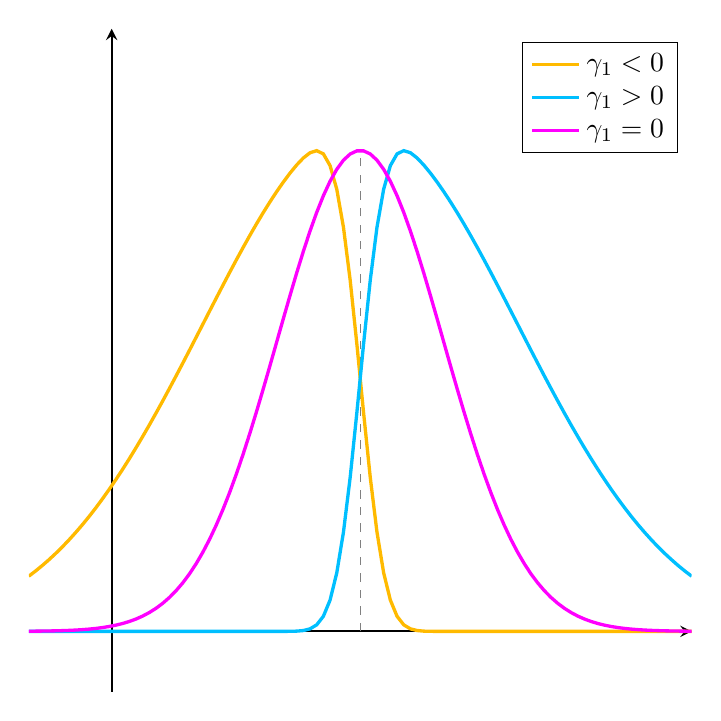
\begin{tikzpicture}
    \begin{axis}[skewkurt, ymax=0.5]
        \draw [dashed,black!50] (3,0) -- (3,0.4);
        \addplot[very thick, color1, samples=100,domain=-1:7] {sknorm(x,3,1.9,-8)};
        \addlegendentry{$\gamma_1<0$}
        \addplot[very thick, color2, samples=100,domain=-1:7] {sknorm(x,3,1.9,8)};
        \addlegendentry{$\gamma_1>0$}
        \addplot[very thick, color3, samples=100,domain=-1:7] {sknorm(x,3,1,0)};
        \addlegendentry{$\gamma_1=0$}
    \end{axis}
    \end{tikzpicture}
    \end{center}
\end{defn}

\begin{defn}
    {\it Коэффициент эксцесса} случайной величины $\xi$:
    \begin{equation*}
        \gamma_2=\mathbb{E}\left(\frac{\xi - \mathbb{E}\xi}{\sqrt{\mathbb{D}\xi}}\right)^4 - 3 = \frac{\mu^4}{\sigma^4} - 3
    \end{equation*}
    Характеризует <<островершинность>> графика плотности распределения:
    \medskip\hfill\break
    \begin{center}
    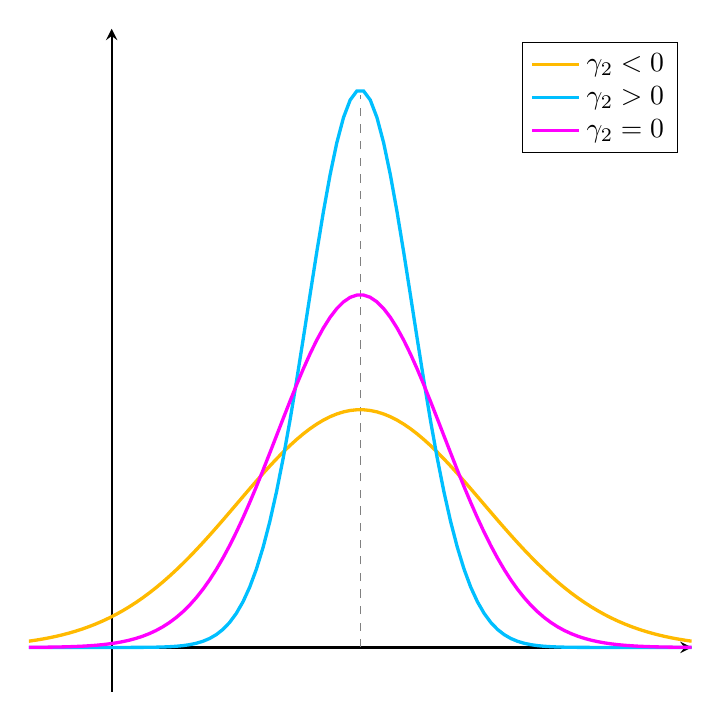
\begin{tikzpicture}
    \begin{axis}[skewkurt]
        \draw [dashed,black!50] (3,0) -- (3,0.625);
        \addplot[very thick, color1, samples=100,domain=-1:7] {normal(x,2.2,3)};
        \addlegendentry{$\gamma_2<0$}
        \addplot[very thick, color2, samples=100,domain=-1:7] {normal(x,0.4,3)};
        \addlegendentry{$\gamma_2>0$}
        \addplot[very thick, color3, samples=100,domain=-1:7] {normal(x,1,3)};
        \addlegendentry{$\gamma_2=0$}
    \end{axis}
    \end{tikzpicture}
    \end{center}
\end{defn}

\begin{rmrk}
    Слагаемое $-3$ добавлено, чтобы коэффициент эксцесса стандартного нормального распределения был равен нулю. Иногда его не учитывают и считают, что коэффициент эксцесса $\mathrm{N}(0,1)$ равен 3.
\end{rmrk}

\iffalse
\medskip\hfill\break
    \begin{center}
    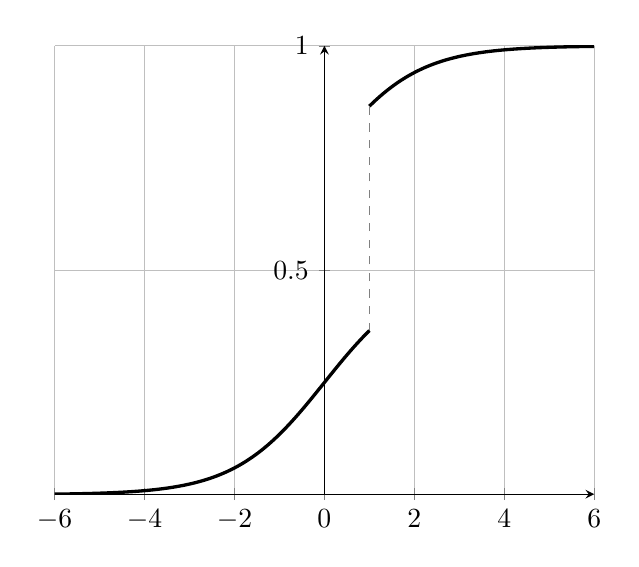
\begin{tikzpicture}[declare function={sigma(\x)=1/(1+exp(-\x));}]
\begin{axis}
[
    grid=major,     
    xmin=-6,
    xmax=6,
    axis x line=bottom,
    ytick={0,.5,1},
    ymax=1,
    axis y line=middle,
    samples=100,
    domain=-6:6,
    legend style={at={(1,0.9)}}     
]
    \draw [dashed,black!50] (1,0.365) -- (1,0.865);
    \addplot[very thick,black,mark=none, samples=100,domain=-6:1]   (x, {.5 * sigma(x)});
    \addplot[very thick,black,mark=none, samples=100,domain=1:6]   (x, {.5 + .5 * sigma(x)});
\end{axis}
\end{tikzpicture}
    \end{center}
\fi

\section {Числовые характеристики случайных величин: квантили. Медиана и ее свойства. Интерквартильный размах}

\begin{defn}
    {\it Медианой} $\operatorname{Med} \xi$ распределения случайной величины $\xi$ называется любое из {\it чисел} $\mu$ таких, что
    \begin{equation*}
        \myprob{\xi \leqslant \mu} \geqslant \frac{1}{2}, ~~~ \myprob{\xi \geqslant \mu} \geqslant \frac{1}{2}.
    \end{equation*}
\end{defn} 

\begin{rmrk}
    Медиана распределения всегда существует, но может быть не единственна, к примеру, в случае дискретного распределения.
\end{rmrk} 

\begin{defn}
{ \itКвантиль порядка $\gamma$} ~--- это такое число $\kappa_\gamma$, для которого выполняется 
$$ \begin{cases} \myprob{\xi \leqslant \kappa_\gamma} = F(\kappa_\gamma) \geqslant \gamma, \\
\myprob{\xi \geqslant \kappa_\gamma} = 1 - F(\kappa_\gamma) \geqslant 1 - \gamma \end{cases}
$$
\end{defn}

\begin{rmrk}
    Если функция распределения $F$ непрерывна и строго монотонна, то {\it квантилем} уровня (порядка) $\gamma$, где $\gamma \in (0; 1), $ является решение $x_\gamma$ уравнения $F(x_\gamma) = \gamma.$ 
    Тогда квантиль порядка $\gamma$ отрезает от области под графиком плотности область с площадью $\gamma$ слева от себя. Справа от $\kappa_\gamma$ площадь области равна $1 - \gamma$.
    
    Если же случайная величина не является абсолютно непрерывной, то уравнение $F(x_\gamma) = \gamma$ может не иметь решений. Например, для приведенного ниже графика не существует $x_{\frac{1}{2}}: F(x_{\frac{1}{2}}) = \frac{1}{2}$.
        
    \medskip\hfill\break
    \begin{center}
    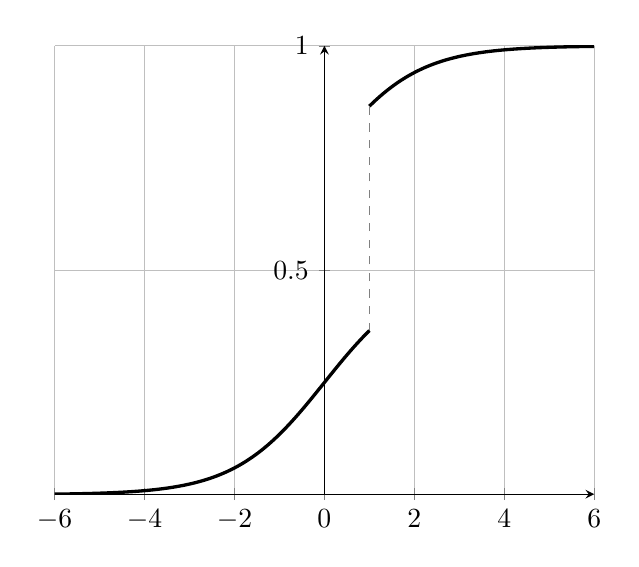
\begin{tikzpicture}[declare function={sigma(\x)=1/(1+exp(-\x));}]
    \begin{axis}
    [
        grid=major,     
        xmin=-6,
        xmax=6,
        axis x line=bottom,
        ytick={0,.5,1},
        ymax=1,
        axis y line=middle,
        samples=100,
        domain=-6:6,
        legend style={at={(1,0.9)}}     
    ]
        \draw [dashed,black!50] (1,0.365) -- (1,0.865);
        \addplot[very thick,black,mark=none, samples=100,domain=-6:1]   (x, {.5 * sigma(x)});
        \addplot[very thick,black,mark=none, samples=100,domain=1:6]   (x, {.5 + .5 * sigma(x)});
    \end{axis}
    \end{tikzpicture}
    \end{center}
\end{rmrk} 

\begin{defn}
    Квантили уровней, кратных $0.01$, называют {\it процентилями}, квантили уровней, кратных $0.1$, — {\it децилями}, уровней, кратных $0.25$, — {\it квартилями}.
\end{defn} 

\begin{rmrk}
    Медиана является квантилем уровня $1 / 2$.
\end{rmrk} 

\begin{namedthm}[Свойства медианы]\leavevmode
\begin{enumerate}
    \item Медиана случайной величины $\xi$ минимизирует средний модуль её отклонения:
    \begin{equation*}
        \mathbb{E}|\xi - \operatorname{Med} \xi| 
    = \min _{a} \mathbb{E}|\xi-a|;
    \end{equation*}
    \item Отклонение медианы случайной величины $\xi$ от её математического ожидания $\mathbb{E}\xi$ не превышает по модулю среднеквадратичного отклонения $\sigma = \sqrt{\mathbb{D}\xi}$:
    \begin{equation*}
        |\mathbb{E}\xi - \operatorname{Med}\xi| \leqslant \sigma.
    \end{equation*}
\end{enumerate}
\end{namedthm}

\begin{proof}
    \begin{enumerate}
        \item Рассмотрим случайную величину $\eta = \xi - \operatorname{Med}\xi$. Очевидно, что $\operatorname{Med} \eta = 0$. Тогда нам надо показать, что $\forall c \in \mathbb{R} $ справедливо 
        \begin{equation*}
            \mathbb{E} |\eta - c| - \mathbb{E}|\eta| \geqslant 0.
        \end{equation*}
        
        Рассмотрим случай $c > 0$. Заметим, что 
        \begin{gather*}
            |\eta - c| - |\eta| = c, \quad \eta < 0 \\
            |\eta - c| - |\eta|  \geqslant -c, \quad \eta \geqslant 0.
        \end{gather*}
        Тогда
        \begin{gather*}
            \mathbb{E} \bigl(|\eta - c| - |\eta| \bigl) 
            = \mathbb{E} \bigl( (|\eta - c| - |\eta|) \cdot \mathrm{I}(\eta < 0) + (|\eta - c| - |\eta|) \cdot \mathrm{I}(\eta \geqslant 0) \bigl) \\
            \mathbb{E} \bigl( |\eta - c| - |\eta| \bigl) \geqslant c~\mathbb{P}(\eta < 0) - c~\mathbb{P}(\eta \geqslant 0).
        \end{gather*}
        Так как $\operatorname{Med}\eta = 0$, то $\mathbb{P}(\eta \leqslant 0) = \mathbb{P}(\eta \geqslant 0) = \frac{1}{2}$.
        Отсюда вытекает
        \begin{equation*}
            \mathbb{E}\bigl( |\eta - c| - |\eta| \bigl) \geqslant 0.
        \end{equation*}
        Случай $c < 0$ сводится к предыдущему умножением случайной величины и $c$ на $-1$. Отсюда следует, что медиана действительно минимизирует средний модуль отклонения.
        \item Рассмотрим цепочку неравенств:
        \begin{multline*}
            |\mathbb{E}\xi - \operatorname{Med}\xi| =
            |\mathbb{E}\left[ \operatorname{Med}\xi - \xi \right]| \leqslant 
            {\text{\{шестое мат. ожидания\}}} \\ \leqslant \mathbb{E} |\operatorname{Med}\xi - \xi|
            \leqslant {\text{\{первое свойство медианы\}}} \\ \leqslant
            \mathbb{E}| \mathbb{E}\xi - \xi| \leqslant
            {\text{\{неравенство Йенсена\}}} \\ 
            \leqslant
            \sqrt{\mathbb{E}| \mathbb{E}\xi - \xi|^2} = 
            \sqrt{\mathbb{D}\xi} = \sigma.
        \end{multline*}
    \end{enumerate}
\end{proof}

\subsubsection{Интерквантильный размах}

\begin{defn}
    {\it Интерквартильным размахом} называется разность между третьим и первым квартилями, то есть ${\displaystyle x_{0{,}75}-x_{0{,}25}}.$
\end{defn} 

В каком-то смысле эту величину можно считать аналогом дисперсии случайной величины, устойчивой к выбросам.

\section {Испытания Бернулли. Биномиальное распределение. Теорема Пуассона. Распределение Пуассона}
\begin{defn}
    {\it Схема Бернулли}~--- последовательность независимых испытаний, в каждом из которых возможны лишь два исхода~--- <<успех>> и <<неудача>>, при этом успех в каждом испытании происходит с одной и той же вероятностью $p \in (0;1)$, а неудача~--- с вероятностью $q = 1 - p.$
\end{defn}

\begin{namedthm}[Формула Бернулли]
Пусть $\xi$~--- случайная величина, равная числу успехов в $n$ испытаниях. Тогда $\forall k = \overline{1,n}$ вероятность получить в $n$ испытаниях ровно $k$ успехов равна
\begin{equation*}
    \mathbb{P}\left(\xi=k\right)=C_{n}^{k} p^{k} q^{n-k}
\end{equation*}
\end{namedthm}

\begin{proof}
Рассмотрим один элементарный исход события $A = \{\xi = k \}$:
\begin{equation*}
    (\underbrace{y, y, \ldots, y}_{k}, \underbrace{\text{\it н}, \text{\it н}, \ldots,\text{\it н}}_{n-k})
\end{equation*}
когда первые $k$ испытаний завершились успехом (у), остальные неудачей (н). Поскольку испытания независимы, вероятность такого элементарного исхода равна $p^k(1 - p)^{n-k}.$ Другие элементарные исходы из события $A$ отличаются лишь расположением $k$ успехов на $n$ местах. Поэтому событие $A$ состоит из $C_n^k$ элементарых исходов, вероятность каждого из которых равна $p^kq^{n-k}$.
\end{proof}

\begin{defn}
    Пусть $\xi_1, \ldots, \xi_n$~--- последовательность независимых случайных величин, имеющих одинаковое распределение Бернулли с параметром $p$ ($\mathbf{Bi}(p)$), то есть принимает значение $1$ (<<успех>>) с вероятностью $p$ и $0$ (<<неудача>>) с вероятностью $1 - p = q$. Тогда говорят, что случайная величина $\xi = \xi_1 + \ldots + \xi_n$ имеет {\it биномиальное распределение} с параметрами $n$ и $p$ ($\mathbf{B}(n, p)$).
\end{defn}

\subsubsection{Числовые характеристики $\mathbf{Bi}(p)$}
\begin{enumerate}
    \item Математическое ожидание:
    \begin{equation*}
        \mathbb{E}\xi =  1 \cdot p + 0 \cdot q = p
    \end{equation*}
    \item Дисперсия:
        $$\mathbb{E}\xi^2 = 1^2 \cdot p + 0^2 \cdot q = p; \quad \mathbb{D}\xi = \mathbb{E}\xi^2 - (\mathbb{E}\xi)^2 = p - p^2 = p \cdot (1 - p) = pq$$
\end{enumerate}

\subsubsection{Числовые характеристики $\mathbf{B}(n, p)$}
\begin{enumerate}
    \item Математическое ожидание:
    \begin{equation*}
        \mathbb{E}\xi = \mathbb{E}(\xi_1 + \ldots + \xi_n) = \mathbb{E}\xi_1 + \ldots + \mathbb{E}\xi_n = \underbrace{p + \ldots + p}_{n} = np
    \end{equation*}
    \item Дисперсия:
    \begin{equation*}
        \mathbb{D}\xi = \mathbb{D}(\xi_1 + \ldots + \xi_n) = \mathbb{D}\xi_1 + \ldots + \mathbb{D}\xi_n = \underbrace{p \cdot q + \ldots + p \cdot q}_{n} = npq
    \end{equation*}
\end{enumerate}

\begin{namedthm}[Теорема Пуассона]
    Пусть проводится $n$ обобщённых испытаний Бернулли (т.е. вероятность успеха испытания зависит от $n$) с вероятностью успеха $p_n$, $\xi$~--- количество успехов в этих испытаниях и $n p_{n} \underset{n \to +\infty}{\longrightarrow} \lambda$. Тогда
    \begin{equation*}
        \forall k \in \mathbb{Z},~ 0 \leqslant k \leqslant n: \quad \mathbb{P}\left(\xi=k\right) \underset{n \to +\infty}{\longrightarrow} \frac{\lambda^{k}}{k !} e^{-\lambda}
    \end{equation*}
\end{namedthm}

\begin{proof}
    По условию теоремы, $n p_n \xrightarrow[n \to +\infty]{} \lambda$. Тогда $p_n \xrightarrow[n \to +\infty]{} 0$. Рассмотрим формулу Бернулли:
    \begin{multline*}
        \mathbb{P}(\xi = k) = C_n^k p^k (1 - p)^{n-k} = \frac{n!}{k!(n - k)!} \cdot \frac{\lambda^k}{n^k} \cdot \left(1 - \frac{\lambda}{n}\right)^{-k} \cdot \left(1 - \frac{\lambda}{n}\right)^n = \\
        = \frac{\lambda^k}{k!} \cdot \frac{(n - k + 1) \cdot \ldots \cdot (n - 1) \cdot n}{n^k} \cdot \left(1 - \frac{\lambda}{n}\right)^n \cdot \left(1 - \frac{\lambda}{n}\right)^{-k}
    \end{multline*}
    Перейдём к пределу при $n \to +\infty$:
    \begin{equation*}
        \frac{(n - k + 1) \cdot \ldots \cdot (n - 1) \cdot n}{n^k} \to 1,~ \left(1 - \frac{\lambda}{n}\right)^n \to e^{-\lambda},~ \left(1 - \frac{\lambda}{n}\right)^{-k} \to 1
    \end{equation*}
    
    Таким образом, получим
    \begin{equation*}
        \mathbb{P}(\xi = k) \xrightarrow[n \to +\infty]{} \frac{\lambda^k}{k!} e^{-\lambda}
    \end{equation*}
\end{proof}

\begin{defn}
    Набор вероятностей $\{\frac{\lambda^k}{k!} e^{-\lambda} \}$, где $k$ принимает значения $0, 1, 2, \ldots$, называется {\it распределением Пуассона} с параметром $\lambda > 0$ ($\mathbf{Pois}(\lambda)$).
\end{defn}
\begin{rmrk}
    Распределение Пуассона представляет собой число событий, произошедших за фиксированное время, при условии, что данные события происходят с некоторой фиксированной средней интенсивностью (за которую отвечает параметр $\lambda$) и независимо друг от друга.
\end{rmrk}

\subsubsection{Числовые характеристики $\mathbf{Pois}(\lambda)$}
\begin{enumerate}
    \item Математическое ожидание:
    \begin{align*}
        \sum\limits_{k=0}^{\infty} e^{-\lambda} \frac{\lambda^k}{k!} = e^{-\lambda} \sum\limits_{k=0}^{\infty} \frac{\lambda^k}{k!} = e^{-\lambda} e^\lambda = 1 \\
        \mathbb{E}\xi = \sum\limits_{k=1}^{\infty} k e^{-\lambda} \frac{\lambda^k}{k!} = e^{-\lambda} \lambda \underbrace{\sum\limits_{k=1}^{\infty} \frac{\lambda^{k-1}}{(k - 1)!}}_{= e^\lambda} = \lambda
    \end{align*}
    \item Дисперсия:
    \begin{align*}
        \mathbb{E}\xi(\xi - 1) = \sum\limits_{k=0}^{\infty} k (k - 1) \frac{\lambda^k}{k!} e^{-\lambda}  = \lambda^2 e^{-\lambda} \sum\limits_{k=2}^{\infty} \frac{\lambda^{k-2}}{(k-2)!} = \lambda^2 e^{-\lambda} e^\lambda = \lambda^2 \\
        \mathbb{E}\xi^2 = \mathbb{E}\xi(\xi - 1) + \mathbb{E}\xi = \lambda^2 + \lambda \quad \Rightarrow \quad \mathbb{D}\xi = \mathbb{E}\xi^2 - (\mathbb{E}\xi)^2 = \lambda
    \end{align*}
\end{enumerate}

\section{Испытания Бернулли. Геометрическое распределение. Теорема Реньи. Показательное распределение}
Рассмотрим схему экспериментов Бернулли с вероятностью успеха $p$, неудачи~--- $q = 1 - p$. Вероятность того, что первый успех произойдёт в испытании с номером $k \in \mathbb{N}$, очевидно, равна $\myprob{\tau = k} = pq^{k-1}$.

\begin{defn}
    Набор вероятностей $\{p q^{k-1}\}$, где $k$ принимает любые значения из множества натуральных чисел, называется {\it геометрическим распределением} вероятностей ($\mathbf{Geom}(p)$).
\end{defn}

Аналогично можно ввести геометрическое распределение как <<число неудач до первого успеха>>. Тогда $k$ будем принимать значения из множества $\{0, 1, 2, \ldots\}$.

\subsubsection{Числовые характеристики $\mathbf{Geom}(p)$}
\begin{enumerate}
    \item Математическое ожидание:
    \begin{multline*}
        \mathbb{E} \xi=\sum\limits_{k=1}^{\infty} k p q^{k-1}=p \sum\limits_{k=1}^{\infty} k q^{k-1}=p \sum\limits_{k=1}^{\infty} \frac{d q^{k}}{d q} = \\
        = p \frac{d}{d q}\left(\sum\limits_{k=1}^{\infty} q^{k}\right)=p \frac{d}{d q}\left(\frac{q}{1-q}\right)=p \frac{1}{(1-q)^{2}}=\frac{1}{p}
    \end{multline*}
    \item Дисперсия:
    \begin{multline*}
        \mathbb{E} \xi(\xi-1)=\sum\limits_{k=1}^{\infty} k(k-1) p q^{k-1}=p q \sum\limits_{k=0}^{\infty} \frac{d^{2} q^{k}}{d q^{2}} =p q \frac{d^{2}}{d q^{2}}\left(\sum\limits_{k=0}^{\infty} q^{k}\right) = \\
        =p q \frac{d^{2}}{d q^{2}}\left(\frac{1}{1-q}\right)=p q \frac{2}{(1-q)^{3}}=\frac{2 q}{p^{2}} \\
        \mathbb{D} \xi=\mathbb{E} \xi(\xi-1)+\mathbb{E} \xi-(\mathbb{E} \xi)^{2}=\frac{2 q}{p^{2}}+\frac{1}{p}-\frac{1}{p^{2}}=\frac{2 q-1+p}{p^{2}}=\frac{q}{p^{2}}
    \end{multline*}
\end{enumerate}

\begin{rmrk}
    Если определять геометрическое распределение как количество неудач до первого успеха, его математическое ожидание изменится:
    \begin{multline*}
        \mathbb{E} \xi=\sum\limits^{\infty}_{\color{red}k=0} k p q^{\color{red}k}= {\color{red}q}p \sum\limits_{k=1}^{\infty} k q^{k-1}= {\color{red}q}p \sum\limits_{k=1}^{\infty} \frac{d q^{k}}{d q} = \\
        = {\color{red}q}p \frac{d}{d q}\left(\sum\limits_{k=1}^{\infty} q^{k}\right)={\color{red}q} p \frac{d}{d q}\left(\frac{q}{1-q}\right)= {\color{red}q}p \frac{1}{(1-q)^{2}}=\frac{{\color{red}q}}{p}
    \end{multline*}
    Так как $q \in (0,1)$, математическое ожидание станет меньше, и это логично ~--- ведь количество неудач до первого успеха всегда на единицу меньше номера первого успеха. (Используя это наблюдение, можно посчитать мат. ожидание ещё проще ~--- $\mathbb{E}(\xi - 1) = \frac{1}{p} - 1 = \frac{1-p}{p} = \frac{q}{p}$). Дисперсия же не зависит от сдвига и останется прежней.
\end{rmrk}

\begin{defn}
    Случайная величина $\xi$ имеет {\it показательное (экспоненциальное) распределение} с параметром $\lambda > 0$ ($\mathbf{Exp}(\lambda)$), если $\xi$ имеет следующие плотность и функцию распределения:
    \begin{equation*}
        f(x) = 
        \begin{cases}
            0, & \text{если $x < 0$;} \\
            \lambda e^{-\lambda x}, & \text{если $x \geqslant 0$.}
        \end{cases}
        \quad 
        F(x) = 
        \begin{cases}
            0, & \text{если $x < 0$;} \\
            1 - e^{-\lambda x}, & \text{если $x \geqslant 0$.}
        \end{cases}
    \end{equation*}
\end{defn}

\begin{rmrk}
    Показательное распределение моделирует время между двумя последовательными свершениями одного и того же события. К примеру, пусть есть магазин, в который время от времени заходят покупатели. При определённых допущениях время между появлениями двух последовательных покупателей будет случайной величиной с экспоненциальным распределением. Среднее время ожидания нового покупателя равно $\frac{1}{\lambda}$. Сам параметр $\lambda$ тогда может быть интерпретирован как среднее число новых покупателей за единицу времени. 
\end{rmrk}

\subsubsection{Числовые характеристики $\mathbf{Exp}(\lambda)$}

Найдём для произвольного $k \in \mathbb{N}$ момент порядка $k$:
\begin{equation*}
    \mathbb{E} \xi^{k}=\int\limits_{-\infty}^{\infty} x^{k} f_{\xi}(x) d x=\int\limits_{0}^{\infty} x^{k} \lambda e^{-\lambda x} d x=\frac{1}{\lambda^{k}} \int\limits_{0}^{\infty}(\lambda x)^{k} e^{-\lambda x} d(\lambda x)=\frac{k !}{\lambda^{k}}
\end{equation*}

В последнем равенстве была использована формула для гамма-функции:
\begin{equation*}
    \Gamma(k+1)=\int\limits_{0}^{\infty} u^{k} e^{-u} d u=k !
\end{equation*}
\begin{enumerate}
    \item Математическое ожидание:
    \begin{equation*}
        \mathbb{E} \xi=\frac{1}{\lambda}
    \end{equation*}
    \item Дисперсия:
    \begin{equation*}
        \mathbb{E} \xi^{2}=\frac{2}{\lambda^{2}}, \quad \mathbb{D} \xi=\mathbb{E} \xi^{2}-(\mathbb{E} \xi)^{2}=\frac{1}{\lambda^{2}}
    \end{equation*}
\end{enumerate}

\begin{thm*}
    Пусть проводится $n$ обобщённых испытаний Бернулли (т.е. вероятность успеха испытания зависит от $n$) с вероятностью успеха $p_n$, $\xi \sim \mathbf{Geom}(p_n)$, $n p_{n} \underset{n \to +\infty}{\longrightarrow} \lambda > 0$. Тогда распределение случайной величины $\frac{\xi}{n}$ сходится к показательному с параметром $\lambda$ при $n \to +\infty$.
\end{thm*}

\begin{proof}
    Пусть $F_n$~--- функция распределения случайной величины $\frac{\xi}{n}$. Тогда для $x \geqslant 0$:
    \begin{equation*}
        F_{n}(x)=\mathbb{P}\left(\frac{\xi_{n}}{n} \leqslant x\right)=\mathbb{P}\left(\xi_{n} \leqslant n x\right)=\mathbb{P}\left(\xi_{n} \leq\lfloor n x\rfloor\right)=1-\left(1-p_{n}\right)^{\lfloor n x\rfloor}
    \end{equation*}
    
    Далее, т.к. $\left(1-p_{n}\right)^{n}=\left(1-\frac{n p_{n}}{n}\right)^{n} \xrightarrow[n \to +\infty]{} e^{-\lambda}$, то $(1 - p_n)^{nx} \xrightarrow[n \to +\infty]{} e^{-\lambda x}.$ По определению, $\lfloor n x\rfloor \leqslant n x<\lfloor n x\rfloor+1$ или, что эквивалентно, $n x-1<\lfloor n x\rfloor \leqslant n x.$ и таким образом верно $(1 - p_n)^{\lfloor nx \rfloor} \xrightarrow[n \to +\infty]{} e^{-\lambda x}$. Следовательно, $F_n(x) \xrightarrow[n \to +\infty]{} 1 - e^{-\lambda x}$, что есть функция показательного распределения. 
\end{proof}

\begin{namedthm}[Теорема Реньи]
Пусть даны случайная величина $N \sim \mathbf{Geom}(p)$, $\xi_1, \xi_2, \ldots$~--- независимые одинаково распределённые случайные величины, $\xi_i \geqslant 0$ и $0 < a = \mathbb{E}\xi < \infty$, $S_n = \sum\limits_{i=1}^N \xi_i$. Тогда
\begin{equation*}
    \sup\limits_{x}\left|\mathbb{P}\left(\frac{p}{a} S_{N}<x\right)-G(x)\right| \underset{p \rightarrow 0}{\longrightarrow} 0,
\end{equation*}

где $G(x)=\left(1-e^{-x}\right) I_{x \geqslant 0}$~--- функция стандартного показательного распределения $\mathbf{Exp}(1)$.

Если $b^2 = \mathbb{E}\xi_i^2$, тогда
\begin{equation*}
    \sup\limits_{x}\left|\mathbb{P}\left(\frac{p}{a} S_{N}<x\right)-G(x)\right| \leqslant \frac{p b^{2}}{(1-p) a^{2}}
\end{equation*}
\end{namedthm}

\section{Испытания Бернулли. Теорема Муавра"--~Лапласа. Нормальное распределение}

\begin{namedthm} [Локальная предельная теорема Муавра"--~Лапласа]
    Пусть $S_n$ - число успехов в $n$ испытаниях Бернулли с вероятностью успеха $0 < p < 1$. Пусть $n \to \infty$, тогда $n p(1-p) {\longrightarrow} \infty$, и 
$$\forall m \in \mathbb{Z}: 0 \leqslant m \leqslant n \quad \mathbb{P}\left(S_{n}=m\right)=\frac{1}{\sigma \sqrt{2 \pi} } e^{-\frac{x^{2}}{2}}\left(1+\underline{O}\left(\frac{1}{\sigma}\right)\right),$$
где $x = \frac{m - np}{\sigma},$ а $\sigma=\sqrt{\mathbb{D} S_{n}}=\sqrt{n p(1-p)}$.
\end{namedthm}  

\begin{namedthm}[Интегральная теорема Муавра"--~Лапласа]
Если выполнено условие локальной теоремы и $C$ - произвольная положительная константа, то равномерно по $a$ и $b$ из отрезка $[-C,C]$ (пусть $b \geqslant a$)
$$\mathbb{P}\left(a \leqslant \frac{S_{n}-n p}{\sqrt{n p(1-p)}} \leqslant b\right) \underset{n \to +\infty}{\longrightarrow} \frac{1}{\sqrt{2 \pi}} \int\limits_{a}^{b} e^{-\frac{x^{2}}{2}} d x.$$
\end{namedthm} 

\begin{defn}
    Случайная величина $\xi$ имеет {\it нормальное (гауссовское) распределение} с параметрами $a$ и $\sigma^2$, где $a \in \mathbb{R}, \sigma > 0$, если $\xi$ имеет следующую плотность распределения: 
$$f(x)=\frac{1}{\sigma \sqrt{2 \pi}} e^{-\frac{(x-a)^{2}}{2 \sigma^{2}}}, \quad x \in \mathbb{R}.$$
\end{defn}

\subsubsection{Матожидание и дисперсия нормального распределения}

Найдем матожидание и дисперсию для {\it стандартного} нормального распределения, т.е. для нормального распределения с параметрами $\alpha = 0$ и $\sigma^2 = 1$:
%$$\mathbb{E} \xi=\int\limits_{-\infty}^{\infty} x f_{\xi}(x) %d x=\frac{1}{\sqrt{2 \pi}} \int\limits_{-\infty}^{\infty} x %e^{-x^{2} / 2} d x=0,$$
\begin{equation*}
    \mathbb{E}\xi = 
    \int\limits_{-\infty}^{\infty} x f_{\xi}(x) dx =
    \frac{1}{\sqrt{2\pi}} \int\limits_{-\infty}^{\infty} x e^{\frac{-x^2}{2}} dx = 
    -\frac{1}{\sqrt{2\pi}} \int\limits_{-\infty}^{\infty} d\left( e^{\frac{-x^2}{2}}\right) = 
    \left. -e^{\frac{-x^2}{2}}\right|_{-\infty}^{\infty} = 0
\end{equation*}

%так как под интегралом стоит нечётная функция. Далее,
Далее, 
\begin{multline*}
    \mathbb{E} \xi^{2}=\frac{1}{\sqrt{2 \pi}} \int\limits_{-\infty}^{\infty} x^{2} e^{-x^{2} / 2} d x=\frac{2}{\sqrt{2 \pi}} \int\limits_{0}^{\infty} x^{2} e^{-x^{2} / 2} d x=-\frac{2}{\sqrt{2 \pi}} \int\limits_{0}^{\infty} x d e^{-x^{2} / 2}= \\
    =-\left.\frac{2 x}{\sqrt{2 \pi}} e^{-x^{2} / 2}\right|_{0} ^{\infty}+2 \int\limits_{0}^{\infty} \frac{1}{\sqrt{2 \pi}} e^{-x^{2} / 2} d x=0+\int\limits_{-\infty}^{\infty} \frac{1}{\sqrt{2 \pi}} e^{-x^{2} / 2} d x=1.
\end{multline*}

Поэтому $\mathbb{D}\xi = \mathbb{E}\xi^2 - (\mathbb{E}\xi)^2 = 1 - 0 = 1.$

Теперь рассмотрим случайную величину $\eta$ с нормальным распределением в общем виде (с параметрами $\alpha$ и $\sigma^2$). Тогда $\xi = \frac{\eta - \alpha}{\sigma}$ - случайная величина со {\it стандартным} нормальным распределением. Далее, т.к. $\mathbb{E}\xi = 0$, $\mathbb{D}\xi = 1$, то 
\begin{gather*}
    \mathbb{E}\eta = \mathbb{E}(\sigma \xi + \alpha) = \sigma \mathbb{E} \xi + \alpha = \alpha, \\
    \mathbb{D}\eta = \mathbb{D}(\sigma \xi + \alpha) = \sigma^2 \mathbb{D}\xi = \sigma^2.
\end{gather*}

\section{Совокупности случайных величин. Совместная функция распределения. Независимость случайных величин. Критерии независимости. Ковариация, коэффициент корреляции}

\subsubsection{Совместное распределение, его свойства}

Пусть случайные величины $\xi_1, \ldots, \xi_n$ заданы на одном вероятностном пространстве $(\Omega, \mathcal{F}, \mathbb{P})$.
\begin{defn}
    {\it Совместное распределение} случайных величин $(\xi_1, \ldots, \xi_n)$~--- функция $\mathbb{P}: \mathfrak{B}(\mathbb{R}^{n}) \to \mathbb{R}^{n}$:
    \begin{equation*}
        \mathbb{P}(\xi \in B) = \mathbb{P}(\omega \colon (\xi_{1}(\omega), \ldots, \xi_{n}(\omega)) \in B),~ B \subset \mathfrak{B}(\mathbb{R}^{n})
    \end{equation*}
\end{defn}
\begin{defn}
    {\it Функция совместного распределения} случайных величин $(\xi_1, \ldots, \xi_n)$~--- функция $F: \mathbb{R}^{n} \to \mathbb{R}^{n}$:
    \begin{equation*}
        F(x_{1}, \ldots, x_{n})=\mathbb{P}(\xi_{1}<x_{1}, \ldots, \xi_{n}<x_{n})
    \end{equation*}
\end{defn}

\begin{rmrk}
    Для функции совместного распределения выполняются свойства, аналогичные одномерному случаю. При этом частные функции распределения восстанавливаются по совместной следующим образом:
    \begin{equation*}
        \lim_{\substack{x_{k} \to +\infty \\ k \neq i}}  F(x_{1}, \ldots, x_{i}, \ldots, x_{n}) = F_{i}(x), \quad i = \overline{1,n}
    \end{equation*}
\end{rmrk}
Далее рассматриваем совместные распределения двух случайных величин.

\subsubsection{Виды многомерных распределений}

\begin{defn}
    Случайные величины $\xi_1, \xi_2$ имеют дискретное совместное распределение, если существует не более чем счётный набор пар неотрицательных чисел $\{a_{i}, b_{j}\}$ такой, что
    \begin{equation*}
        \sum\limits_{i=1}^{\infty} \sum\limits_{j=1}^{\infty} \mathbb{P}\left(\xi_{1}=a_{i}, \xi_{2}=b_{j}\right)=1
    \end{equation*}
    Таблицу, на пересечении $i$-й строки и $j$-го столбца которой стоит вероятность $\mathbb{P}\left(\xi_{1}=a_{i}, \xi_{2}=b_{j}\right)$, называют {\it таблицей совместного распределения} случайных величин $\xi_1$ и $\xi_2$.
\end{defn}
\begin{defn}
    Случайные величины $\xi_1, \xi_2$ имеют абсолютно непрерывное совместное распределение, если существует неотрицательная функция $f_{\xi_{1}, \xi_{2}}(x, y)$ такая, что для любого борелевского множества $B \in \mathfrak{B}\left(\mathbb{R}^{2}\right)$ имеет место равенство
    \begin{equation*}
        \mathbb{P}\left(\left(\xi_{1}, \xi_{2}\right) \in B\right)=\iint\limits_{B} f_{\xi_{1}, \xi_{2}}(x, y) d x d y
    \end{equation*}
    Если такая функция $f_{\xi_{1}, \xi_{2}}(x, y)$ существует, она называется {\it плотностью совместного распределения} случайных величин $\xi_1, \xi_2$.
    
    Функция совместного распределения в этом случае имеет вид:
    \begin{equation*}
        F(x, y)=\mathbb{P}(\xi_{1}<x, \xi_{2}<y)=\int\limits_{-\infty}^{x}\left(\int\limits_{-\infty}^{y} f_{\xi_{1}, \xi_{2}}(u, v) d v\right) d u
    \end{equation*}
\end{defn}

\begin{rmrk}
    Плотность совместного распределения имеет те же свойства, что и плотность распределения одной случайной величины: неотрицательность и нормированность:
    \begin{equation*}
        f(x, y) \geqslant 0~ \forall x,y \in \mathbb{R}; \quad \iint\limits_{\mathbb{R}^{2}} f(x, y) dx dy = 1
    \end{equation*}

    По функции совместного распределения его плотность находится как смешанная частная производная (в точках, где она существует):
    \begin{equation*}
        f(x, y)=\frac{\partial^{2}}{\partial x \partial y} F(x, y)
    \end{equation*}
\end{rmrk}

\begin{rmrk}
    Из существования плотностей $\xi_1$ и $\xi_2$ не следует абсолютная непрерывность совместного распределения этих случайных величин. Например, вектор $(\xi, \xi)$ принимает значения только на диагонали в $\mathbb{R}^2$ и уже поэтому не имеет плотности распределения (его распределение сингулярно). Обратное же свойство, как показывает следующая теорема, всегда верно.
\end{rmrk}

\begin{thm*}
    Если случайные величины $\xi_1$ и $\xi_2$ имеют абсолютно непрерывное совместное распределение с плотностью $f(x, y)$, то $\xi_1$ и $\xi_2$ в отдельности также имеют абсолютно непрерывное распределение с плотностями:
    \begin{equation*}
        f_{\xi_{1}}(x)=\int\limits_{-\infty}^{\infty} f(x, y) d y ; \quad f_{\xi_{2}}(y)=\int\limits_{-\infty}^{\infty} f(x, y) d x
    \end{equation*}
    Для $n > 2$ плотности случайных величин $\xi_1, \ldots, \xi_n$ находятся по плотности их совместного распределения $f(x_1, \ldots, x_n)$ интегрированием функции $f$ по всем <<лишним>> координатам.
\end{thm*}
\begin{proof}
\begin{equation*}
    F_{\xi_{1}}\left(x_{1}\right)
    = \lim _{x_{2} \rightarrow+\infty} F_{\xi_{1}, \xi_{2}}\left(x_{1}, x_{2}\right)
    = \int\limits_{-\infty}^{x_{1}}\left(\int\limits_{-\infty}^{\infty} f(x, y) d y\right) d x
    = \int\limits_{-\infty}^{x_{1}} f_{\xi_{1}}(x) d x
\end{equation*}
\end{proof}

\subsubsection{Независимость случайных величин}
\begin{defn}
    Случайные величины $\xi_1, \ldots, \xi_n$ называют {\it независимыми в совокупности}, если для любого набора борелевских множеств $B_{1}, \ldots, B_{n} \in \mathfrak{B}(\mathbb{R})$:
    \begin{equation*}
        \mathbb{P}\left(\xi_{1} \in B_{1}, \ldots, \xi_{n} \in B_{n}\right)=\mathbb{P}\left(\xi_{1} \in B_{1}\right) \cdot \ldots \cdot \mathbb{P}\left(\xi_{n} \in B_{n}\right)
    \end{equation*}
\end{defn}
\begin{namedthm}[Критерий независимости]
    Случайные величины $\xi_1, \ldots, \xi_n$ независимы в совокупности $\Leftrightarrow$ имеет место равенство:
    \begin{equation*}
        F_{\xi_{1}, \ldots, \xi_{n}}\left(x_{1}, \ldots, x_{n}\right)=F_{\xi_{1}}\left(x_{1}\right) \cdot \ldots \cdot F_{\xi_{n}}\left(x_{n}\right)
    \end{equation*}
    В частности, в случае дискретного совместного распределения:
    \begin{equation*}
        \mathbb{P}\left(\xi_{1}=a_{1}, \ldots, \xi_{n}=a_{n}\right)=\mathbb{P}\left(\xi_{1}=a_{1}\right) \cdot \ldots \cdot \mathbb{P}\left(\xi_{n}=a_{n}\right) \quad \forall a_1, \ldots, a_n \in \mathbb{R}
    \end{equation*}
    В случае абсолютно непрерывного:
    \begin{equation*}
        f_{\xi_{1}, \ldots, \xi_{n}}\left(x_{1}, \ldots, x_{n}\right)=f_{\xi_{1}}\left(x_{1}\right) \cdot \ldots \cdot f_{\xi_{n}}\left(x_{n}\right)
    \end{equation*}
\end{namedthm}

\subsubsection{Формула свёртки}

Пусть $\xi_1, \xi_2$~--- случайные величины с плотностью совместного распределения $f_{\xi_{1}, \xi_{2}}\left(x_{1}, x_{2}\right)$, задана борелевская функция $g: \mathbb{R}^{2} \rightarrow \mathbb{R}$. Требуется найти функцию распределения (и плотность, если она существует) случайной величины $\eta=g\left(\xi_{1}, \xi_{2}\right)$.
\begin{lem}
    Пусть $x \in \mathbb{R}$, задана область $D_{x} \subseteq \mathbb{R}^{2},~ D_x = \{(u,v): g(u,v) < x\}$ Тогда случайная величина $\eta=g\left(\xi_{1}, \xi_{2}\right)$ имеет функцию распределения
    \begin{equation*}
        F_{\eta}(x)=\mathbb{P}\left(g\left(\xi_{1}, \xi_{2}\right)<x\right)=\mathbb{P}\left(\left(\xi_{1}, \xi_{2}\right) \in D_{x}\right)=\iint\limits_{D_{x}} f_{\xi_{1}, \xi_{2}}(u, v) d u d v
    \end{equation*}
\end{lem}
Далее считаем, что случайные величины $\xi_1$ и $\xi_2$ независимы, т. е. $f_{\xi_{1}, \xi_{2}}(u, v) \equiv f_{\xi_{1}}(u) f_{\xi_{2}}(v)$. В этом случае распределение величины $g\left(\xi_{1}, \xi_{2}\right)$ полностью определяется частными распределениями величин $\xi_1$ и $\xi_2$.
\begin{namedthm}[Формула свёртки]
    Если случайные величины $\xi_1$ и $\xi_2$ независимы и имеют абсолютно непрерывные распределения с плотностями $f_{\xi_{1}}(u)$ и $f_{\xi_{2}}(v)$, то плотность распределения суммы $\xi_{1}+\xi_{2}$ существует и равна <<свёртке>> плотностей $f_{\xi_{1}}$ и $f_{\xi_{2}}$:
    \begin{equation*}
        f_{\xi_{1}+\xi_{2}}(t)=\int\limits_{-\infty}^{\infty} f_{\xi_{1}}(u) f_{\xi_{2}}(t-u) d u=\int\limits_{-\infty}^{\infty} f_{\xi_{2}}(u) f_{\xi_{1}}(t-u) d u
    \end{equation*}
\end{namedthm}

\begin{proof}
    Воспользуемся утверждением вышеуказанной леммы для борелевской функции $g(u, v)=u+v$. Интегрирование по двумерной области $D_{x}=\{(u, v) \colon u+v<x\}$ можно заменить последовательным вычислением двух интегралов: наружного — по переменной $u$, меняющейся в пределах от $-\infty$ до $+\infty$, и внутреннего~--- по переменной $v$, которая при каждом $u$ должна быть меньше, чем $x-u$. Поэтому
    \begin{equation*}
        F_{\xi_{1}+\xi_{2}}(x)=\iint\limits_{D_{x}} f_{\xi_{1}}(u) f_{\xi_{2}}(v) d v d u=\int\limits_{-\infty}^{\infty}\left(\int\limits_{-\infty}^{x-u} f_{\xi_{1}}(u) f_{\xi_{2}}(v) d v\right) d u
    \end{equation*}
    
    Сделаем в последнем интеграле замену $v=t-u$. При этом $v \in(-\infty, x-u) \Leftrightarrow t \in(-\infty, x), d v=d t$. В полученном интеграле меняем порядок интегрирования:
    \begin{equation*}
        F_{\xi_{1}+\xi_{2}}(x)=\int\limits_{-\infty}^{\infty} \int\limits_{-\infty}^{x} f_{\xi_{1}}(u) f_{\xi_{2}}(t-u) d t d u=\int\limits_{-\infty}^{x}\left(\int\limits_{-\infty}^{\infty} f_{\xi_{1}}(u) f_{\xi_{2}}(t-u) d u\right) d t
    \end{equation*}
    Из функции распределения $F_{\xi_{1}+\xi_{2}}(x)$ выражается плотность $f_{\xi_{1}+\xi_{2}}(t)$.
\end{proof}

\subsubsection{Ковариация, коэффициент корреляции, их свойства}

Рассмотрим случайные величины $\xi$ и $\eta$. Дисперсия их суммы в общем случае равна
\begin{equation*}
    \mathbb{D}(\xi+\mathrm{n})=\mathbb{D} \xi+\mathbb{D} \eta+2(\mathbb{E}(\xi \eta)-\mathbb{E} \xi \mathbb{E} \eta)
\end{equation*}
\begin{defn}
    Величина $\mathbb{E}(\xi \eta)-\mathbb{E} \xi \mathbb{E} \eta = \operatorname{cov}(\xi, \eta)$ называется {\it ковариацией} случайных величин $\xi$ и $\eta$.
\end{defn}
Если $\xi$ и $\eta$ независимы, то $\operatorname{cov}(\xi, \eta) = 0$. Обратное, вообще говоря, неверно.
\begin{exmp}
    Рассмотрим $\xi \sim \mathbf{U}[0;1]$, случайные величины $\eta_{1}=\cos \xi$ и $\eta_{2}=\sin \xi$.
    \begin{enumerate}
        \item Докажем некореллированность данных случайных величин.
        \begin{gather*}
            \mathbb{E} \eta_{1}=\int\limits_{-\pi}^{\pi} \cos x \cdot \frac{1}{2 \pi} d x=0, \quad \mathbb{E} \eta_{2}=\int\limits_{-\pi}^{\pi} \sin x \cdot \frac{1}{2 \pi} d x=0 \\
            \mathbb{E} \eta_{1} \eta_{2}=\int\limits_{-\pi}^{\pi}(\cos x \sin x) \frac{1}{2 \pi} d x=\frac{1}{4 \pi} \int\limits_{-\pi}^{\pi} \sin 2 x d x=0
        \end{gather*}
        Следовательно, $\operatorname{cov}(\eta_1, \eta_2) = 0$
        \item Докажем зависимость $\eta_1$ и $\eta_2$. Рассмотрим события:
        \begin{equation*}
            A = \left\{\omega \colon \eta_1(\omega) \in \left[0, \frac{1}{2} \right] \right\}, \quad
            B = \left\{\omega \colon \eta_2(\omega) \in \left[0, \frac{1}{2} \right] \right\},
        \end{equation*}
        Проверим по критерию независимости:
        \begin{gather*}
            \mathbb{P}\left\{\eta_{1} \in\left[0, \frac{1}{2}\right]\right\}=\mathbb{P}\left\{\xi \in\left[-\frac{\pi}{2},-\frac{\pi}{3}\right] \cup\left[\frac{\pi}{3}, \frac{\pi}{2}\right]\right\}=\frac{1}{2 \pi} \cdot 2 \cdot \frac{\pi}{6}=\frac{1}{6} \\
            \mathbb{P}\left\{\eta_{2} \in\left[0, \frac{1}{2}\right]\right\}=\mathbb{P}\left\{\xi \in\left[0, \frac{\pi}{6}\right] \cup\left[\frac{5 \pi}{6}, \pi\right]\right\}=\frac{1}{2 \pi} \cdot 2 \cdot \frac{\pi}{6}=\frac{1}{6} \\
            \mathbb{P}\left\{\eta_{1} \in\left[0, \frac{1}{2}\right], \eta_{2} \in\left[0, \frac{1}{2}\right]\right\}=\mathbb{P}\{\varnothing\}=0 \neq \frac{1}{6} \cdot \frac{1}{6}
        \end{gather*}
        Следовательно, $\eta_1$ и $\eta_2$~--- зависимы.
    \end{enumerate}
\end{exmp}

\begin{namedthm}[Свойства ковариации]\leavevmode
    \begin{enumerate}
        \item $\operatorname{cov}(\xi, \xi)=\mathbb{D} \xi$;
        \item $\operatorname{cov}(\xi, \eta)=\operatorname{cov}(\eta, \xi)$;
        \item $\operatorname{cov}(a \xi + b, \eta)=a \operatorname{cov}(\xi, \eta)$, если $a, b \in \mathbb{R}$;
        \item $\operatorname{cov}(\eta + \zeta, \xi) = 
        \operatorname{cov}(\eta, \xi) + \operatorname{cov}(\zeta, \xi)$;
        \item $\operatorname{cov}^2(\xi, \eta) \leqslant \mathbb{D}\xi \, \mathbb{D}\eta$,
        
        $\operatorname{cov}^2(\xi, \eta) = \mathbb{D}\xi \,\mathbb{D}\eta \; \Leftrightarrow \; \xi \overset{\text{п.н.}}{=} a\eta + b, \; a, b \in \mathbb{R}$;
        
        (Аналог неравенства Коши-Буняковского)
    \end{enumerate}
\end{namedthm}

Величина ковариации характеризует меру (линейной) зависимости случайных величин. Однако от умножения на константу (не равную нулю) зависимость случайных величин не изменяется никак, в отличие от ковариации. Введём новый термин.

\begin{defn}
    {\it Коэффициент корреляции} $\rho(\xi,\eta)$ случайных величин $\xi$ и $\eta$, дисперсии которых существуют и отличны от нуля:
    \begin{equation*}
        \rho(\xi, \eta)=\frac{\operatorname{cov}(\xi, \eta)}{\sqrt{\mathbb{D} \xi} \sqrt{\mathbb{D} \eta}}
    \end{equation*}
\end{defn}

\begin{namedthm}[Свойства коэффициента корреляции]\leavevmode
    \begin{enumerate}
        \item Коэффициент корреляции независимых случайных величин равен нулю.
        \item Для любых двух случайных величин (для которых выполнены условия определения) их коэффициент корреляции по модулю не превосходит единицы.
        \item Если $|\rho(X,Y)| = 1$, то с вероятностью один $X$ и $Y$ линейно выражаются друг через друга. То есть,
        \begin{equation*}
            |\rho(X, Y)|=1 \Longrightarrow \exists \: b \neq 0, \, c \in \mathbb{R}: \mathbb{P}(X-b Y=c)=1
        \end{equation*}
        При этом знак коэффициента $b$ совпадает со знаком коэффициента корреляции.
    \end{enumerate}
\end{namedthm}

\begin{proof}
    \begin{enumerate}
    \item В числителе дроби, которой равен коэффициент корреляции,
окажется ноль. В знаменателе нуля быть не должно, это обеспечивается определением.

    \item  Обозначим эти две случайные величины как $\xi$ и $\eta$ и центрируем: $\xi_c = \xi - \mathbb{E}\xi$ и $\eta_c = \eta - \mathbb{E}\eta$. Так как $\operatorname{cov}(\xi, \eta)=\operatorname{cov}\left(\xi_{c}, \eta_{c}\right)$, а дисперсия случайной величины не меняется от смещения случайной величины на константу, коэффициент корреляции не изменится.
    
    Далее, т.к. $\mathbb{E} \xi_{c}=\mathbb{E} \eta_{c}=0$:
    \begin{gather*}
        \mathbb{D} \xi_{c}=\mathbb{E} \xi_{c}^{2}-\left(\mathbb{E} \xi_{c}\right)^{2}=\mathbb{E} \xi_{c}^{2},~ \mathbb{D} \eta_{c}=\mathbb{E} \eta_{c}^{2} \\
        \operatorname{cov}\left(\xi_{c}, \eta_{c}\right)=\mathbb{E}\left(\xi_{c} \eta_{c}\right)-\mathbb{E} \xi_{c} \mathbb{E} \eta_{c}=\mathbb{E}\left(\xi_{c} \eta_{c}\right)
    \end{gather*}
    
    Далее идут те же рассуждения, что часто используются при доказательстве неравенства Коши-Буняковского:
    \begin{equation*}
        \forall a \in \mathbb{R} \quad 0 \leqslant \mathbb{D}\left(\xi_{c}-a \eta_{c}\right)=\mathbb{E}\left(\xi_{c}-a \eta_{c}\right)^{2}-\left(\mathbb{E}\left(\xi_{c}-a \eta_{c}\right)\right)^{2}=\mathbb{E}\left(\xi_{c}-a \eta_{c}\right)^{2}
    \end{equation*}
    
    Полученное неравенство можно рассматривать как квадратное неравенство относительно $a$, а именно
    \begin{equation*}
        \mathbb{E}\left(\xi_{c}-a \eta_{c}\right)^{2}=\mathbb{E} \xi_{c}^{2}-2 a \mathbb{E}\left(\xi_{c} \eta_{c}\right)+a^{2} \mathbb{E} \eta_{c}^{2} \geqslant 0
    \end{equation*}
    
    Поскольку верно это для любого $a$, то дискриминанту нельзя быть больше нуля. То есть:
    \begin{multline*}
        \left(\mathbb{E}\left(\xi_{c} \eta_{c}\right)\right)^{2}-\mathbb{E} \xi_{c}^{2} \mathbb{E} \eta_{c}^{2} \leqslant 0 \Longleftrightarrow\left|\mathbb{E}\left(\xi_{c} \eta_{c}\right)\right| \leqslant \sqrt{\mathbb{E} \xi_{c}^{2} \mathbb{E} \eta_{c}^{2}} \Rightarrow \\
        \Rightarrow\left|\operatorname{cov}\left(\xi_{c}, \eta_{c}\right)\right| \leqslant \sqrt{\mathbb{D} \xi_{c} \mathbb{D} \eta_{c}}
    \end{multline*}
    
    По доказанному выше <<стирание>> индексов не изменит коэффициентов.

    \item Доказательство этого свойства целиком опирается на доказательство предыдущего: если выполнилось равенство $|\operatorname{cov}(\xi, \eta)|=\sqrt{\mathbb{D} \xi \mathbb{D} \eta}$, то квадратное неравенство относительно $a$ может обращаться в равенство при некотором $a = b$. Но это равенство означает, что равна нулю $\mathbb{D}(\xi-b \eta)$, а это сразу говорит о том, что с вероятностью один $\xi - b\eta$ равна константе. Обозначим эту константу за $c$ и получим то, что нужно было доказать.
    
    Знак коэффициента корреляции совпадает с знаком ковариации, так дисперсии по предположению положительны. Выразив $\xi$ через $\eta$, мы можем воспользоваться свойствами ковариации и получить
    $$ \rho(\xi, \eta) = \rho(b\eta + c, \eta)=
    \frac{\operatorname{cov}(b\eta + c, \eta)}
    {\sqrt{\mathbb{D}(b\eta + c) \, \mathbb{D}\eta}} = 
    \frac{b\operatorname{cov}(\eta, \eta)}
    {\sqrt{b^2\, \mathbb{D}\eta \, \mathbb{D}\eta}} = 
    \frac{b\mathbb{D}\eta}
    {|b|\mathbb{D}\eta} = 
    \text{sign}(b).
    $$

\end{enumerate}
\end{proof}

\section{Виды сходимости последовательностей случайных величин}
\begin{defn}
    Последовательность случайных величин $\{\xi_n\}$ {\it почти наверное сходится} к случайной величине $\xi$ ($\xi_n \xrightarrow[]{\text{п.н.}} \xi$), если
    \begin{equation*}
        \mathbb{P}\left(\left\{\omega \colon \lim\limits _{n \rightarrow \infty} \xi_{n}(w)=\xi(w)\right\}\right)=1.
    \end{equation*}
\end{defn}

\begin{defn}
    Последовательность случайных величин $\{\xi_n\}$ {\it сходится по вероятности} к случайной величине $\xi$ ($\xi_n \xrightarrow[]{\text{p}} \xi$), если
    \begin{equation*}
        \forall \varepsilon>0 \quad P\left(\left\{\omega \colon |\xi_{n}(\omega)-\xi(\omega)|>\varepsilon\right\}\right) \xrightarrow[n \to +\infty]{} 0.
    \end{equation*}
\end{defn}

\begin{defn}
    Последовательность случайных величин $\{\xi_n\}$ {\it сходится в среднем} к случайной величине $\xi$ ($\xi_n \xrightarrow[]{\text{(r)}} \xi$), если
    \begin{equation*}
        \mathbb{E}\left|\xi_{n}-\xi\right|^{r} \xrightarrow[n \to +\infty]{} 0.
    \end{equation*}
\end{defn}

\begin{defn}
    Последовательность случайных величин $\{\xi_n\}$ {\it сходится по распределению} к случайной величине $\xi$ ($\xi_n \xrightarrow[]{\text{d}} \xi$), если
    \begin{equation*}
        F_{\xi n}(x) \xrightarrow[n \to +\infty]{} F_{\xi}(x) \quad \forall x, \, \text{в которых}~ F_{\xi} ~\text{непрерывна}.
    \end{equation*}
\end{defn}

\begin{defn}
    Последовательность случайных величин $\{\xi_n\}$ {\it слабо сходится} к случайной величине $\xi$ ($\xi_n \stackrel{\text{w}}{\Rightarrow} \xi$), если
    \begin{equation*}
        \mathbb{E} f\left(\xi_{n}\right) \rightarrow \mathbb{E} f(\xi) \quad \forall~ \text{непрерывной ограниченной}~ f(x).
    \end{equation*}
\end{defn}
\begin{thm*}
    Вышеуказанные виды сходимости последовательностей случайных величин связаны следующими отношениями:
    
    \adjustbox{scale=1.25,center}
    {%
    \begin{tikzcd}[column sep=scriptsize, row sep=tiny]
    \text{п.н.} \arrow[dr, Rightarrow] & &  & \\
    & \text{p} \arrow[r, Rightarrow] & \text{d} \arrow[r, Leftrightarrow] & \text{w} \\
    \text{(r)} \arrow[ur, Rightarrow] & & &
    \end{tikzcd}
   }
\end{thm*}

\begin{proof}
    \begin{itemize}
        \item[$\text{(r)} \Rightarrow \text{p}$] Из \hyperlink{cheb}{обобщённого неравенства Чебышёва}:
    \begin{equation*}
        \mathbb{P}(|\xi_n - \xi| \geqslant \varepsilon) \leqslant \cfrac{\mathbb{E}|\xi_n - \xi|^{r}}{\varepsilon^{r}} \xrightarrow[n \to +\infty]{} 0
    \end{equation*}
    
    \item[$\text{(r)} \nLeftarrow \text{p}$] Рассмотрим последовательность случайных величин:
    \begin{gather*}
        \xi_n = 
        \begin{cases}
            0, & \frac{1}{n} \leqslant \omega \leqslant 1; \\
            \sqrt[r]{n}, & 0 \leqslant \omega \leqslant \frac{1}{n}.
        \end{cases}
        \Rightarrow p_1 = 1 - \frac{1}{n},~ p_2 = \frac{1}{n} \\
        \mathbb{P}(|\xi_n| > \varepsilon) \xrightarrow[n \to +\infty]{} 0,~ \text{однако $~\mathbb{E}|\xi_n|^{r} = 1$}.
    \end{gather*}
    
    \item[$\text{п.н.} \Rightarrow \text{p}$]
    Ограничимся для простоты случаем, когда $\xi_n(\omega) \rightarrow \xi(\omega)$ для любого $\omega$. Зафикисируем $\omega \in \Omega.$ По определению предела, $\xi_n(\omega) \xrightarrow[n \to +\infty]{} \xi(\omega)$, если для всякого $\varepsilon > 0$ найдётся $N = N(\omega, \varepsilon) \geqslant 0$ такое, что для всех $n > N$ выполняется неравенство $|\xi_n(\omega) - \xi(\omega)| < \varepsilon$.
    
    Событие $A = \{n > N(\omega,\varepsilon) \}$ влечёт событие $B = \{|\xi_n(\omega) - \xi(\omega)| < \varepsilon \}$. Тогда 
    $$1 \geqslant \mathbb{P}(B) \geqslant \mathbb{P}(A)=\mathbb{P}(N(\omega, \varepsilon)<n)=F_{N(\varepsilon, \omega)}(n) \xrightarrow[n \to +\infty]{} 1.$$ по свойству функции распределения. Таким образом, было получено, что $\mathbb{P}(B) \rightarrow 1$, т.е. $\xi_n \xrightarrow[]{\text{p}} \xi.$
    
    \item[$\text{п.н.} \nLeftarrow \text{p}$]
    
    Положим $\xi_{2^{k}}=\mathrm{I}\left(\left[0, \frac{1}{2^{k}}\right]\right), \xi_{2^{k}+p}=\mathrm{I}\left(\left[\frac{p}{2^{k}}, \frac{p+1}{2^{k}}\right]\right), 1 \leqslant p<2^{k}.$ Тогда $\xi_n \xrightarrow[]{\text{p}} 0$, т.к. $\mathbb{P}(\xi_n > 0) \leqslant$ длина отрезка в индикаторе $\leqslant \frac{2}{n} \rightarrow 0$, но $\xi_n \overset{\text{п.н.}}{\nrightarrow} 0$, т.к. $\forall \omega \quad \exists$ бесконечно много $n$, таких что $\xi_n(\omega) = 1.$
    
    \item[$\text{(r)} \nRightarrow \text{п.н.}$] См. предыдущий пример.
    
    \item[$\text{(r)} \nLeftarrow \text{п.н.}$]
    
    $\Omega = [0,1], \mathcal{F} = \mathcal{B}([0,1])$, $\mathbb{P}$ - равномерное распределение. Определим для $k \geqslant 1 \quad \xi_k = 2^{k-1} \mathrm{I}\left(\left[0, \frac{1}{2^{k-1}}\right]\right).$ Тогда $\forall k \quad \mathbb{E}\xi_k = 1$, но $\xi = \mathrm{I}(\omega = 0)$.
    
    \item[$\text{p} \Rightarrow \text{w}$]
    
    Пусть $f$ - ограниченная и непрерывная функция, $|f| \leqslant C$. Зафиксируем $\varepsilon > 0$. Т.к. $\mathbb{P}(|\xi| = \infty) = 0$, то $\exists N, \exists \delta$:
    
    \begin{enumerate}
        \item $\mathbb{P}(|\xi| > N) \leqslant \frac{\varepsilon}{6C}$, т.к. $\mathbb{P}(\xi = \infty) = 0$.
        \item $\mathbb{P}(|\xi_n - \xi| > \delta) \leqslant \frac{\varepsilon}{6C}$ из сходимости по вероятности (при достаточно больших $n$).
        \item $\forall x,y |x| < N, |x - y| < \delta|f(x) - f(y)| \leqslant \frac{\varepsilon}{3}$, т.к. $f$ равномерно непрерывна на отрезке $[-N, N]$.
    \end{enumerate}
    
    Рассмотрим следующие события:
    
    $$ A_{1}=\left\{\left|\xi_{n}-\xi\right| \leqslant \delta\right\} \cap\{|\xi|<N\} $$
    $$ A_{2}=\left\{\left|\xi_{n}-\xi\right| \leqslant \delta\right\} \cap\{|\xi| \geqslant N\} $$
    $$ A_{3}=\left\{\left|\xi_{n}-\xi\right|>\delta\right\} $$
    
    Эти события образуют разбиение $\Omega=A_{1} \sqcup A_{2} \sqcup A_{3} $. 
    
    Оценим $|\mathbb{E}f(\xi_n) - \mathbb{E}f(\xi)|$:
    
    $$\left|\mathbb{E} f\left(\xi_{n}\right)-\mathbb{E} f(\xi)\right|=\left|\mathbb{E}\left(f\left(\xi_{n}\right)-f(\xi)\right)|\leqslant 
    \mathbb{E}| f\left(\xi_{n}\right)-f(\xi) |=\right.$$
    $$=\mathbb{E}\left|f\left(\xi_{n}\right)-f(\xi)\right|\left(\mathrm{I}_{A_{1}}+\mathrm{I}_{A_{2}}+\mathrm{I}_{A_{3}}\right) \leq$$
    $$\leqslant \frac{\varepsilon}{3} \mathbb{P}\left(A_{1}\right)+2 C\left(\mathbb{P}\left(A_{2}\right)+\mathbb{P}\left(A_{3}\right)\right) \leqslant \frac{\varepsilon}{3}+2 C\left(\frac{\varepsilon}{6 C}+\frac{\varepsilon}{6 C}\right)=\varepsilon,$$
    
    откуда следует, что $|\mathbb{E}f(\xi_n) - \mathbb{E}f(\xi)| \rightarrow 0 \Rightarrow \xi_n \xrightarrow[]{\text{w}} \xi$.
    
    \item[p $\nLeftarrow d$]
    
    Пусть $\xi_n = \begin{cases}
    1, \; p_1 = \frac{1}{2} \\
    0, \; p_0 = \frac{1}{2}
    \end{cases}, \; 
    \xi = \begin{cases}
    1, \; p_1 = \frac{1}{2} \\
    0, \; p_0 = \frac{1}{2}
    \end{cases}.$ \\
    Тогда $|\xi_n - \xi| = \begin{cases}
    1, \; p_1 = \frac{1}{2} \\
    0, \; p_0 = \frac{1}{2}
    \end{cases},$ \; и не выполняется определение сходимости по вероятности, например, при $\varepsilon_0 = \frac{1}{3}$, т.к. 
    $$ \mathbb{P}\left({|\xi_n - \xi| > \frac{1}{3}}\right) = \frac{1}{2} {\nrightarrow} 0 \text{ при } n \to \infty.
    $$
    
   \item[$\text{p} \nLeftarrow \text{w}$]
    
    Пусть $\Omega = \{\omega_1, \omega_2 \}, \mathbb{P}(\{\omega_i \}) = \frac{1}{2}.$ 
    
    Определим для любого $n$ $\xi_n(\omega_1) = 1, \xi_n(\omega_2) = -1.$ Положим $\xi = -\xi_n.$ Тогда:
    
    $$ \mathbb{E}f(\xi_n) = \frac{f(1) + f(-1)}{2} = \mathbb{E}f(\xi),$$
    
    но $\forall n \quad |\xi_n - \xi| = 2 \Rightarrow \xi_n \overset{\text{p}}{\nrightarrow} \xi.$
    
\end{itemize}    
\end{proof}

\begin{rmrk}
    Cлабая сходимость всё же не есть сходимость случайных величин, и ею нельзя оперировать как сходимостями п.н. и по вероятности, для которых предельная случайная величина единственна (с точностью до значений на множестве нулевой вероятности).
\end{rmrk}

\begin{rmrk}
    Во многих источниках слабая сходимость и сходимость по распределению вводятся как один и тот же вид сходимости. Те немногие доказательства эквивалентности, найденные авторами, либо требуют знания теории меры, либо являются слишком кринжовыми, чтобы включать их в это учебное пособие.
\end{rmrk}

\section{Неравенства Маркова, Чебышёва и Гаусса. Правило «трех сигм». Закон больших чисел в форме Чебышёва}
\begin{namedthm}[Неравенство Маркова]
    Если $\mathbb{E}|\xi| < \infty$, то для любого $x > 0$
    \begin{equation*}
        \myprob{|\xi| \geqslant x} \leqslant \frac{\mathbb{E}|\xi|}{x}
    \end{equation*}
\end{namedthm}

\begin{proof}
\begin{equation*}
    \mathrm{I}(A) \sim \mathbf{Bi}(p),~ p = \myprob{\mathrm{I}(A) = 1} = \myprob{A} = \mathbb{E}\mathrm{I}(A)
\end{equation*}

Индикаторы прямого и противоположного событий связаны равенством $\mathrm{I}(A) + \mathrm{I}(\overline{A}) = 1.$ Поэтому
\begin{equation*}
    |\xi|=|\xi| \cdot \mathrm{I}(|\xi|<x)+|\xi| \cdot \mathrm{I}(|\xi| \geqslant x) \geqslant|\xi| \cdot \mathrm{I}(|\xi| \geqslant x) \geqslant x \cdot \mathrm{I}(|\xi| \geqslant x)
\end{equation*}

Тогда $\mathbb{E}|\xi| \geqslant \mathbb{E}(x \cdot \mathrm{I}(|\xi| \geqslant x))=x \cdot \mathbb{P}(|\xi| \geqslant x)$. Осталось разделить обе части этого неравенства на положительное число $x$.
\end{proof}

\hypertarget{cheb}{}
\begin{crlr}[Обобщённое неравенство Чебышёва] 
Пусть функция $g$ не убывает и неотрицательна на $\mathbb{R}$. Если $\mathbb{E}g(\xi) < \infty$, то для любого $x \in \mathbb{R}$
\begin{equation*}
    \mathbb{P}(\xi \geqslant x) \leqslant \frac{\mathbb{E} g(\xi)}{g(x)}
\end{equation*}
\end{crlr}
\begin{proof}
    Заметим, что $\myprob{\xi \geqslant x} \leqslant \myprob{g(\xi) \geqslant g(x)}$, поскольку функция $g$ не убывает. Оценим последнюю вероятность по неравенству Маркова, которое можно применять в силу неотрицательности $g$
    \begin{equation*}
        \mathbb{P}(g(\xi) \geqslant g(x)) \leqslant \frac{\mathbb{E} g(\xi)}{g(x)}
    \end{equation*}
\end{proof}
\begin{crlr}[Неравенство Чебышёва]
    Если $\mathbb{D}\xi$ существует, то для любого $x > 0$
    \begin{equation*}
        \mathbb{P}(|\xi-\mathbb{E} \xi| \geqslant x) \leqslant \frac{\mathbb{D} \xi}{x^{2}}
    \end{equation*}
\end{crlr}
\begin{proof}
    Для $x > 0$ неравенство $|\xi - \mathbb{E}\xi| \geqslant x \Leftrightarrow (\xi - \mathbb{E}\xi)^2 \geqslant x^2$, поэтому
    \begin{equation*}
        \mathbb{P}(|\xi-\mathbb{E} \xi| \geqslant x)=\mathbb{P}\left((\xi-\mathbb{E} \xi)^{2} \geqslant x^{2}\right) \leqslant \frac{\mathbb{E}(\xi-\mathbb{E} \xi)^{2}}{x^{2}}=\frac{\mathbb{D} \xi}{x^{2}}
    \end{equation*}
\end{proof}
\begin{defn}
    В неравенстве Чебышёва в качестве $x$ можно брать любое положительное число. Если взять в качестве $x$ величину $3\sigma$, где $\sigma$~--- стандартное отклонение (то есть именно корень из дисперсии), то получится
    \begin{equation*}
        \mathbb{P}(|X-\mathbb{E} X|>3 \sigma) \leqslant \frac{\mathbb{D} X}{9 \mathbb{D} X}=\frac{1}{9} \Leftrightarrow \mathbb{P}(|X-\mathbb{E} X| \leqslant 3 \sigma) \geqslant 1-\frac{1}{9}=\frac{8}{9}
    \end{equation*}
    Это соотношение называется {\it правилом трёх сигм}.
\end{defn}

\begin{namedthm}[Неравенство Гаусса]
    Пусть $X$~--- одномодальная случайная величина с модой $m$ и пусть $a^2$ - математическое ожидание $(X - m)^2.$ Тогда
    \begin{equation*}
        \mathbb{P}(|X-m|>k) \leq
        \begin{cases}
            \left(\cfrac{2 a}{3 k}\right)^{2}, & \text{если $k \geqslant \frac{2 a}{\sqrt{3}}$;} \\
            1 - \cfrac{k}{a \sqrt{3}}, & \text{если $0 \leqslant k \leqslant \frac{2 a}{\sqrt{3}}$;}
        \end{cases}
    \end{equation*}
\end{namedthm}

\begin{defn}
    Говорят, что последовательность случайных величин $\xi_1, \xi_2, \ldots$ с конечными первыми моментами {\it удовлетворяет закону больших чисел}, если
    \begin{equation*}
        \frac{\xi_{1}+\ldots+\xi_{n}}{n}-\frac{\mathbb{E} \xi_{1}+\ldots+\mathbb{E} \xi_{n}}{n} \xrightarrow[]{\text{p}} 0 \: \text {при} \: n \to +\infty
    \end{equation*}
\end{defn}
\begin{namedthm}[Закон больших чисел в форме Чебышёва]
    Для любой последовательности $\xi_1, \xi_2, \ldots$ попарно независимых и одинаково распределённых случайных величин с конечным вторым моментом $\mathbb{E}\xi_1^2 < \infty$ имеет место сходимость
    \begin{equation*}
        \frac{\xi_{1}+\ldots+\xi_{n}}{n} \xrightarrow[]{\text{p}} \mathbb{E} \xi_{1}
    \end{equation*}
\end{namedthm}

\begin{proof}
    Обозначим через $S_n = \xi_1 + \ldots + \xi_n$ сумму первых $n$ случайных величин. Из линейности матожидания получим
    \begin{equation*}
        \mathbb{E}\left(\frac{S_{n}}{n}\right)=\frac{\mathbb{E} \xi_{1}+\ldots+\mathbb{E} \xi_{n}}{n}=\frac{n \mathbb{E} \xi_{1}}{n}=\mathbb{E} \xi_{1}
    \end{equation*}
    
    Пусть $\varepsilon > 0.$ Воспользуемся неравенством Чебышёва:
    \begin{multline*}
        \mathbb{P}\left(\left|\frac{S_{n}}{n}-\mathbb{E}\left(\frac{S_{n}}{n}\right)\right| \geqslant \varepsilon\right) \leqslant \frac{\mathbb{D}\left(\frac{S_{n}}{n}\right)}{\varepsilon^{2}}
        = \frac{\mathbb{D} S_{n}}{n^{2} \varepsilon^{2}}
        = \frac{\mathbb{D} \xi_{1}+\ldots+\mathbb{D} \xi_{n}}{n^{2} \varepsilon^{2}}= \\
        = \frac{n \mathbb{D} \xi_{1}}{n^{2} \varepsilon^{2}}
        = \frac{\mathbb{D} \xi_{1}}{n \varepsilon^{2}} \xrightarrow[n \to +\infty]{} 0,
    \end{multline*}
    так как $\mathbb{D}\xi_1 < \infty$. Дисперсия суммы превратилась в сумму дисперсий в силу попарной независимости слагаемых, из-за которой все ковариации $\operatorname{cov}(\xi_i, \xi_j)$ по свойству ковариации обратились в нуль при $i \neq j$.
\end{proof}

\section{Характеристические функции и их свойства}
\begin{defn}
    {\it Характеристическая функция случайной величины} $\xi$~--- функция $\varphi_{\xi}: \mathbb{R} \rightarrow \mathbb{C}$:
    \begin{equation*}
        \varphi_{\xi}(t)
        = \mathbb{E} e^{it \xi}
        = \mathbb{E} \cos (t \xi)+i \mathbb{E} \sin (t \xi) = \int\limits_{\mathbb{R}}^{} e^{i t x} d F_{\xi}(x),
    \end{equation*}
    где интеграл справа называется {\it интегралом Фурье-Стильтьеса}.
    
    Для абсолютно непрерывного распределения характеристическая функция имеет вид
    \begin{equation*}
        \varphi_{\xi}(t)=\int\limits_{\mathbb{R}} e^{i t x} f(x) d x
    \end{equation*}
    Для дискретного, соответственно
    \begin{equation*}
        \varphi_{\xi}(t)=\sum\limits_{i} e^{i t x_{i}} \mathbb{P}\left\{\xi=x_{i}\right\}
    \end{equation*}
\end{defn}

\begin{exmp}
    Характеристическая функция случайной величины $\xi \sim \mathbf{N}(0;1)$:
    \begin{multline*}
        \varphi_{\xi}(t) 
        = \frac{1}{\sqrt{2 \pi}} \int\limits_{-\infty}^{\infty} e^{i t x} e^{-x^{2} / 2} d x
        = \frac{1}{\sqrt{2 \pi}} \int\limits_{-\infty}^{\infty} e^{-t^{2} / 2} e^{-x^2/2 \,+\, itx \,+\, t^2/2} d x = \\
        = \frac{1}{\sqrt{2 \pi}} \int\limits_{-\infty}^{\infty} e^{-t^{2} / 2} e^{-(x-i t)^{2} / 2} d x =  
         e^{-t^{2} / 2} \frac{1}{\sqrt{2 \pi}} \int\limits_{-\infty}^{\infty} e^{-(x-i t)^{2} / 2} d(x-i t)
        = e^{-t^{2} / 2}
    \end{multline*}
\end{exmp}

\begin{namedthm}[Свойства характеристической функции]\leavevmode
    \begin{enumerate}
        \item Характеристическая функция существует для любой случайной величины $\xi$.
        \item $\forall~ \xi,~ \forall~ a, b \in \mathbb{R} \colon \varphi_{a \xi + b}(t) = e^{itb} \varphi_{\xi}(at)$
        \item $|\varphi_{\xi}(t)|=|\mathbb{E} e^{i t \xi}| \leqslant 1,~ \varphi_{\xi}(0) = 1, ~\overline{\varphi_{\xi}(t)} = \varphi_{\xi}(-t) = \varphi_{-\xi}(t) ~\forall t \in \mathbb{R}$
        
        \mycon{}
        Если характеристическая функция вещественнозначна, то она является чётной.
        
        \item Если случайные величины $\xi$ и $\eta$ независимы, то
        \begin{equation*}
            \varphi_{\xi + \eta}(t) = \varphi_{\xi}(t) \varphi_{\eta}(t)
        \end{equation*}
        \item Характеристическая функция равномерно непрерывна.
        \item Если существует абсолютный момент $k$-го порядка $\mathbb{E}|\xi|^{k} < \infty,~ k \geqslant 1$, то существует непрерывная $k$-я производная характеристической функции:
        \begin{equation*}
            \left.\cfrac{\partial^{k} \varphi_{\xi}(t)}{\partial t^{k}}\right|_{t=0}= i^{k} \mathbb{E} \xi^{k}
        \end{equation*}
        
        Если существует непрерывная производная характеристической функции порядка $k = 2n, n \in \mathbb{N}$, то существует абсолютный момент порядка $k = 2n: \; \mathbb{E}|\xi|^k = \mathbb{E}\xi^k$ (а следовательно, и все предыдущие) и его можно вычислить по той же формуле.
        
        \item Характеристическая функция случайно величины $\xi$ однозначно определяет её функцию распределения $F_{\xi}$. Функция распределения восстанавливаются по характеристической функции с помощью обратных преобразований Фурье.
        
        Дискретное распределение:
        \begin{equation*}
            \mathbb{P}(\xi=k)=\frac{1}{2 \pi} \int\limits_{-\pi}^{\pi} e^{-i t k} \varphi_{\xi}(t) d t, k \in \mathbb{Z}
        \end{equation*}
        
        Абсолютно непрерывное распределение:
        \begin{equation*}
            f_{\xi}(x)=\frac{1}{2 \pi} \int\limits_{-\infty}^{\infty} e^{-i t x} \varphi_{\xi}(t) d t, x \in \mathbb{R}
        \end{equation*}
    \item $\xi_n \Rightarrow \xi \Leftrightarrow \varphi_{\xi_{n}}(t) \to \varphi_{\xi}(t)$ (теорема Леви о непрерывном соответствии)
    \end{enumerate}
\end{namedthm}

\begin{proof}
    \begin{enumerate}
        \item Существование характеристической функции равносильно равномерной сходимости соответствующего интеграла. Докажем её по признаку Вейерштрасса:
        \begin{equation*}
            \left|\varphi_{\xi}(t)\right|=\left|\int\limits_{\mathbb{R}} e^{i t x} d F(x)\right| \leqslant \int\limits_{\mathbb{R}}\left|e^{i t x}\right| d F(x)=\int\limits_{\mathbb{R}} d F(x)=1
        \end{equation*}
        \item $\varphi_{a \xi+b}(t) 
        = \mathbb{E}e^{i t(a \xi+b)}
        = e^{i t b} \mathbb{E}e^{i t a \xi}
        = e^{i t b} \varphi_{\xi}(t a)$
        \item Неравенство доказано в пункте 1, первое равенство очевидно.
        \begin{equation*}
            \varphi_{\xi}(-t) = \mathbb{E}cos(-t \xi) + i\mathbb{E}sin(-t \xi) = \mathbb{E}cos(t \xi) - i\mathbb{E}sin(t \xi) = \overline{\varphi_{\xi}(t)}
        \end{equation*}
        Оставшиеся равенства следуют из второго свойства.
        \item $\varphi_{\xi + \eta}(t) 
        = \mathbb{E}e^{it(\xi + \eta)} 
        = \mathbb{E}e^{it\xi}\mathbb{E}e^{it\eta}
        = \varphi_{\xi}(t)\varphi_{\eta}(t)$
        \item Выберем сколь угодно малое $\varepsilon > 0$ и оценим разность значений характеристической функции в точках $t$ и $t + h$:
        \begin{multline*}
            |\varphi(t+h)-\varphi(t)| 
            = \left|\int\limits_{\mathbb{R}} \left(e^{i(t+h) x}-e^{i tx}\right) d F(x)\right|
            = \left|\int\limits_{\mathbb{R}} e^{i t x}\left(e^{i h x}-1\right) d F(x)\right| \leqslant \\
            \leqslant \int\limits_{\mathbb{R}} \left|e^{i h x}-1\right| d F(x)=\int\limits_{|x| \leqslant R}\left|e^{i h x}-1\right| d F(x)+\int\limits_{|x|>R}\left|e^{i h x}-1\right| d F(x)
        \end{multline*}
        Теперь выберем $R$ настолько большим, чтобы $\mathbb{P}(|X|>R) < \frac{\varepsilon}{4}$. Поскольку $\left|e^{i h x}-1\right| \leqslant 2$, второй интеграл при этом не превосходит по величине $\frac{\varepsilon}{2}$. После этого выберем $h$ столь малым, чтобы $\left|e^{i h x}-1\right|<\frac{\varepsilon}{2}~$ при всех $|x| \leqslant R$. Тогда и первый интеграл не превосходит $\frac{\varepsilon}{2}$ и, таким образом, по заданному $\varepsilon > 0$ подобрано столь малое $h >0$, что $|\varphi(t+h)-\varphi(t)|<\varepsilon~ \forall t \in \mathbb{R}$.
        \item Если существует $\mathbb{E}\xi^{k}<\infty,~ k \geqslant 1$, то для всех $m = \overline{1, k}$ существуют $\mathbb{E}\xi^{m}<\infty$. Следовательно,
        \begin{equation*}
            \left|\int\limits_{\mathbb{R}}(i x)^{m} e^{i t x} d F(x)\right| \leqslant \int\limits_{\mathbb{R}}|x|^{k} d F(x)=\mathbb{E}|\xi|^{m}<\infty \quad \forall m = \overline{1, k}
        \end{equation*}
        Т.е. интегралы $\int\limits_{\mathbb{R}}(i x)^{m} e^{i t x} d F(x)$ сходятся равномерно по $t$, а значит, дифференцирование по $t$ можно менять местами с операцией интегрирования, откуда
        \begin{equation*}
            \varphi_{\xi}^{(m)}(t)=i^{m} \int\limits_{\mathbb{R}} x^{m} e^{i t x} d F(x),~ \varphi_{\xi}^{(m)}(0)=i^{m} \int\limits_{\mathbb{R}} x^{m} d F(x)=i^{m} \mathbb{E}\xi^{m}
        \end{equation*}
        
        Пусть у характеристической функции существует непрерывная производная чётного порядка $k$. Характеристическая функция и её производные непрерывны, функция $e^{itx}$ бесконечно (а значит, и нужные нам $k$ раз) дифференцируема по $t$, и можно показать, что при этих условиях можно поменять знаки интегрирования и дифференцирования местами.\footnote{Достаточно обозначить интеграл $\int\limits_{\mathbb{R}}{x^{m} e^{itx}dF(x)}, \, m = \overline{0, k-1}$ за $G(t)$ и расписать его производную по $t$ по определению, воспользовавшись тем, что $\int\limits_{\mathbb{R}} o(\Delta t) dF(x) = o(\Delta t) \int\limits_{\mathbb{R}} dF(x) = o(\Delta t)$.}
        Тогда мы получим, что 
        $$\varphi^{(k)}(0) = i^k \left.\mathbb{E}\xi^k e^{itx}\right|_{t=0} = i^k \mathbb{E}\xi^k = 
        \int\limits_{\mathbb{R}} x^k dF(x)
        $$
        В силу чётности $k ~~ x^k \geqslant 0$, а значит, указанный интеграл сходится абсолютно, что и означает существование искомого математического ожидания.
    \end{enumerate}
\end{proof}

\section{Закон больших чисел в форме Хинчина. Усиленный закон больших чисел в форме Колмогорова}
\begin{namedthm}[Закон больших чисел в форме Хинчина] \leavevmode

    Для любой последовательности $\xi_{1}, \xi_{2}, \ldots$ независимых и одинаково распределённых случайных величин с конечным первым моментом $E\left|\xi_{1}\right|<\infty$ имеет место сходимость:
    \begin{equation*}
        \frac{S_{n}}{n} = \frac{\xi_{1}+\ldots+\xi_{n}}{n} %\xrightarrow[]{\text{p}} \mathbb{E} \xi_{1}
        \stackrel{\text{p}}{\longrightarrow} \mathbb{E}\xi_1
    \end{equation*}
\end{namedthm}
Для доказательства теоремы нам потребуется следующая лемма.
\begin{lem}
    Если $\xi_{n} \Rightarrow c=const$, то $\xi_{n} \xrightarrow[]{\text{p}} c$
\end{lem}
\begin{proof}
    Пусть $\xi_{n} \Rightarrow c$, т.е.
    \begin{equation*}
        F_{\xi_{n}}(x) \rightarrow F_{c}(x) =
        \begin{cases}
            0, & x \leqslant c; \\
            1, & x > c.
        \end{cases}
    \end{equation*}
    при любом $x$, являющемся точкой непрерывности предельной функции $F_{c}(x)$, т. е. $\forall~ x \neq c$.
    
    Возьмём произвольное $\varepsilon>0$ и докажем, что $\mathbb{P}\left(\left|\xi_{n}-c\right|<\varepsilon\right) \rightarrow 1$:
    \begin{multline*}
        \mathbb{P}\left(-\varepsilon<\xi_{n}-c<\varepsilon\right)=\mathbb{P}\left(c-\varepsilon<\xi_{n}<c+\varepsilon\right) \geqslant \mathbb{P}\left(c-\varepsilon / 2 \leqslant \xi_{n}<c+\varepsilon\right)= \\
        \quad=F_{\xi_{n}}(c+\varepsilon)-F_{\xi_{n}}(c-\varepsilon / 2) \rightarrow F_{c}(c+\varepsilon)-F_{c}(c-\varepsilon / 2)=1-0=1
    \end{multline*}
    поскольку в точках $c+\varepsilon$ и $c-\varepsilon / 2$ функция $F_{c}$ непрерывна, и, следовательно, имеет место сходимость последовательностей $F_{\xi_{n}}(c+\varepsilon)$ к $F_{c}(c+\varepsilon)=1$ и $F_{\xi_{n}}(c-\varepsilon / 2)$ к $F_{c}(c-\varepsilon / 2)=0$.
    
    Осталось заметить, что $\mathbb{P}\left(\left|\xi_{n}-c\right|<\varepsilon\right)$ не бывает больше $1$, так что по свойству предела зажатой последовательности $\mathbb{P}\left(\left|\xi_{n}-c\right|<\varepsilon\right) \rightarrow 1$.
\end{proof}

Перейдём к доказательству теоремы.

\begin{proof}
    По вышеприведённому свойству сходимость по вероятности к постоянной эквивалентна слабой сходимости. Так как $a$~--- постоянная, достаточно доказать слабую сходимость $\frac{S_{n}}{n}$ к $a$. По теореме о непрерывном соответствии, эта сходимость имеет место тогда и только тогда, когда для любого $t \in \mathbb{R}$ сходятся характеристические функции
    \begin{equation*}
        \varphi_{S_{n} / n}(t) \rightarrow \varphi_{a}(t)=\mathbb{E} e^{i t a}=e^{i t a}
    \end{equation*}
    
    Найдём характеристическую функцию случайной величины $\frac{S_{n}}{n}$. Пользуясь свойствами характеристической функции, получаем
    \begin{equation*}
        \varphi_{S_{n} / n}(t)=\varphi_{S_{n}}\left(\frac{t}{n}\right)=\left(\varphi_{\xi_{1}}\left(\frac{t}{n}\right)\right)^{n}
    \end{equation*}
    
    Вспомним, что первый момент $\xi_{1}$ существует, поэтому мы можем разложить $\varphi_{\xi_{1}}(t)$ в ряд Тейлора в окрестности нуля:
    \begin{equation*}
        \varphi_{\xi_{1}}(t)=1+i t \mathbb{E} \xi_{1}+o(|t|)=1+i t a+o(|t|)
    \end{equation*}
    
    В точке $\frac{t}{n}$ соответственно:
    \begin{gather*}
        \varphi_{\xi_{1}}\left(\frac{t}{n}\right)=1+\frac{i t a}{n}+o\left(\left|\frac{t}{n}\right|\right) \\
        \varphi_{S_{n} / n}(t)=\left(\varphi_{\xi_{1}}\left(\frac{t}{n}\right)\right)^{n}=\left(1+\frac{i t a}{n}+o\left(\left|\frac{t}{n}\right|\right)\right)^{n}
    \end{gather*}
    
    При $n \to +\infty$ воспользуемся <<замечательным пределом>> $\left(1+\frac{x}{n}\right)^{n} \rightarrow e^{x}$ и получим:
    \begin{equation*}
        \varphi_{S_{n} / n}(t)=\left(1+\frac{i t a}{n}+o\left(\left|\frac{t}{n}\right|\right)\right)^{n} \rightarrow e^{i t a}
    \end{equation*}
\end{proof}

\hypertarget{SLLN}{}
\begin{namedthm}[Усиленный закон больших чисел в форме Колмогорова]
Пусть $\xi_1, \xi_2, \ldots, \xi_n, \ldots, $ ~--- независимые одинаково распределённые случайные величины (сокращённо н.о.р.с.в.). Тогда 
\begin{enumerate}
    \item Если существует $\mathbb{E}{\xi_1} = a$, то $\displaystyle \myprob{\lim\limits_{n \to \infty} \cfrac{1}{n} \sum\limits_{i = 1}^n \xi_i = a} = 1$. 
    
    Иными словами, $\displaystyle \cfrac{1}{n} \sum\limits_{i = 1}^n \xi_i \stackrel{\text{п.н.}}{\longrightarrow} a $.
    
    \item Если существует $\displaystyle \lim\limits_{n \to \infty} \cfrac{1}{n} \sum\limits_{i = 1}^n \xi_i = a$, то существует $\mathbb{E}\xi_1 = a$.
\end{enumerate}
\end{namedthm}

\section{Центральная предельная теорема}
\begin{namedthm}[Центральная предельная теорема]
    Пусть $\xi_{1}, \xi_{2}, \ldots$~--- последовательность независимых одинаково распределенных (невырожденных) случайных величин с $\mathbb{E} \xi_{1}^{2}<\infty$ и $S_{n}=\xi_{1}+\ldots+\xi_{n}$. Тогда
    \begin{equation*}
        \mathbb{P}\left(\frac{S_{n}-\mathbb{E} S_{n}}{\sqrt{\mathbb{D} S_{n}}} \leqslant x\right)
        \xrightarrow[n \to +\infty]{}
        \Phi(x) = \frac{1}{\sqrt{2 \pi}} \int\limits_{-\infty}^{x} e^{-\frac{z^{2}}{2}} dz~ \forall x \in \mathbb{R}
    \end{equation*}
\end{namedthm}
\begin{proof}
Пусть $\mathbb{E} \xi_{1}=m,\, \mathbb{D} \xi_{1}=\sigma^{2}$. Введём $X = \xi_1 - m$ и $\varphi_X(t)=\mathbb{E} e^{i tX}$. Введём также
\begin{equation*}
    \varphi_{n}(t)=\mathbb{E} e^{i t \frac{S_{n}-\mathbb{E} S_{n}}{\sqrt{\mathbb{D} S_{n}}}} = 
    \left[\varphi_X\left(\frac{t}{\sigma \sqrt{n}}\right)\right]^{n}
\end{equation*}

В силу разложения характеристической функции
\begin{equation*}
    \varphi_{X}(t)=1+i t \mathbb{E} X+\ldots+\frac{(i t)^{n}}{n !} \mathbb{E} X^{n}+R_{n}(t)
\end{equation*}

При $n=2$ получим 
\begin{equation*}
    \varphi(t)=1-\frac{\sigma^{2} t^{2}}{2}+\overline{o}\left(t^{2}\right), \quad t \rightarrow 0
\end{equation*}

Следовательно, для любого $t \in \mathbb{R}$ при $n \to +\infty$
\begin{equation*}
    \varphi_{n}(t)=\left[1-\frac{\sigma^{2} t^{2}}{2 \sigma^{2} n}+\overline{o}\left(\frac{1}{n}\right)\right]^n \rightarrow e^{-\frac{t^{2}}{2}}
\end{equation*}

Функция $e^{-\frac{t^{2}}{2}}$ является характеристической функцией $\mathbf{N}(0,1)$. В силу теорем о непрерывном соответсвии между функциями распределения и характеристическими функциями центральная предельная теорема доказана.
\end{proof}

\section{Условное математическое ожидание}

Пусть $\xi$ и $\eta$~--- две случайные величины на некотором вероятностном пространстве, причём $E|\xi|<\infty$; $L=L(\eta)$~--- множество, в котором собраны все случайные величины, имеющие вид $\zeta=g(\eta)$, где $g(x)$~--- произвольная борелевская функция. Скалярным произведением двух случайных величин $\varphi$ и $\zeta$ назовём $(\varphi, \zeta)=\mathbb{E}(\varphi \cdot \zeta)$, если это математическое ожидание существует.

Условное математическое ожидание $\mathbb{E}(\xi | \eta)$ случайной величины $\xi$ относительно $\eta$ можно представлять себе как результат ортогонального проектирования случайной величины $\xi$ на пространство $L$.

Результат проектирования — такая случайная величина $\mathbb{E}(\xi | \eta)=\widehat{\xi}$, для которой выполнено основное и единственное свойство ортопроекции: её разность с $\xi$ ортогональна всем элементам $L$. Ортогональность означает, что для любой $g(\eta) \in L$ обращается в нуль (если вообще существует) скалярное произведение $(\xi-\widehat{\xi}, g(\eta))$, т. е.
\begin{equation*}
    \mathbb{E}((\xi-\widehat{\xi}) g(\eta))=0~ \text{или}~ \mathbb{E}(\xi g(\eta))=\mathbb{E}(\widehat{\xi} g(\eta))
\end{equation*}
Это свойство называют {\it тождеством ортопроекции}. Чтобы матожидание существовало всегда, достаточно брать лишь ограниченные функции $g(y)$.

\begin{defn}
    Пусть $\mathbb{E}|\xi|<\infty$, $L=L(\eta)$~--- множество всех борелевских функций от случайной величины $\eta$. Условным математическим ожиданием $\mathbb{E}(\xi | \eta)$ называется случайная величина $\widehat{\xi} \in L$, удовлетворяющая тождеству ортопроекции.
\end{defn}

\begin{namedthm}[Свойства условного математического ожидания]\leavevmode
    \begin{enumerate}
        \item Все свойства математического ожидания, как, например, линейность, сохраняются, однако борелевские функции от случайной величины $\eta$ выносятся из-под знака математического ожидания как постоянные.
        \item Пусть $\mathbb{E} \xi^{2}<\infty$.Тогда расстояние от $\xi$ до её ортопроекции $\widehat{\xi}=\mathbb{E}(\xi | \eta)$ является наименьшим из расстояний от $\xi$ до всех «точек» множества $L$:
        \begin{equation*}
            \min_{g(\eta) \in L} \mathbb{E}(\xi-g(\eta))^{2}=\mathbb{E}(\xi-\widehat{\xi})^{2}
        \end{equation*}
        \item Если $f(\eta) \in L$ такова, что $\mathbb{E}|f(\eta) \cdot \xi|<\infty$, то
        \begin{equation*}
            \mathbb{E}(f(\eta) \cdot \xi | \eta)
            \stackrel{\text{п.н.}}{=}
            f(\eta) \cdot \mathbb{E}(\xi | \eta)
        \end{equation*}
        \begin{proof}
            Рассмотрим только случай, когда $f(\eta)$ ограничена. Проверим, что $\zeta=f(\eta) \cdot \mathbb{E}(\xi | \eta)$ удовлетворяет тождеству ортопроекции: для любой ограниченной $g(\eta) \in L$
            \begin{equation*}
                \mathbb{E}(f(\eta) \xi \cdot g(\eta))=\mathbb{E}(\zeta \cdot g(\eta))
            \end{equation*}
            Обозначим $h(\eta)=f(\eta) g(\eta) \in L$. Эта функция ограничена, поэтому
            \begin{equation*}
                \mathbb{E}(\xi f(\eta) \cdot g(\eta))=\mathbb{E}(\xi h(\eta))=\mathbb{E}(\widehat{\xi} h(\eta))=\mathbb{E}(\zeta \cdot g(\eta))
            \end{equation*}
        \end{proof}
        \item Если $\mathbb{E}|g(\xi, \eta)|<\infty$, то
        \begin{equation*}
            \mathbb{E} g(\xi, \eta)=\mathbb{E}\left[\left.\mathbb{E}(g(\xi, y) | \eta)\right|_{y=\eta}\right]
        \end{equation*}
        \item Если $\xi$ и $\eta$ независимы, то $\mathbb{E}(\xi | \eta)=\mathbb{E} \xi$.
    \end{enumerate}
\end{namedthm}

\subsubsection{Вычисление условного матожидания}
Возьмём функцию $h(y)=\mathbb{E}(\xi \,|\, \eta=y)$, для которой $\mathbb{E}(\xi | \eta)=h(\eta)$ и рассмотрим, что такое условное математическое ожидание относительно события $\{\eta=y\}$ для двух случаев: когда обе случайные величины имеют дискретное распределение и когда их совместное распределение абсолютно непрерывно.
\begin{enumerate}
    \item Пусть $\xi$ принимает значения $a_{1}, a_{2}, \ldots$, а $\eta$~--- значения $b_{1}, b_{2}, \ldots$ Тогда $h(\eta)$ может принимать только значения $h\left(b_{1}\right), h\left(b_{2}\right), \ldots$, где
    \begin{equation*}
        h(y)=\sum\limits_{i} a_{i} \mathbb{P}\left(\xi=a_{i} | \eta=y\right)
    \end{equation*}
    Иначе говоря, при каждом фиксированном $y$ начение $h(y)$ определяется как математическое ожидание дискретного распределения со значениями $a_{i}$ и вероятностями $\mathbb{P}\left(\xi=a_{i} | \eta=y\right)$. Такое распределение называется {\it условным распределением случайной величины $\xi$ при условии $\eta = y$}.
    
    \item Во втором случае пусть $f_{\xi, \eta}(x, y)$~--- плотность совместного распределения, $f_{\eta}(y)$~--- плотность распределения величины $\eta$.Тогда положим
    \begin{equation*}
        h(y)=\int\limits_{\mathbb{R}} x \frac{f_{\xi, \eta}(x, y)}{f_{\eta}(y)} d x
    \end{equation*}
    При фиксированном $y$ число $h(y)$ есть математическое ожидание абсолютно непрерывного распределения с плотностью распределения
    \begin{equation*}
        f(x | y)=\frac{f_{\xi, \eta}(x, y)}{f_{\eta}(y)}=\frac{f_{\xi, \eta}(x, y)}{\int\limits_{\mathbb{R}} f_{\xi, \eta}(x, y) d x}
    \end{equation*}
    Такое распределение называется {\it условным распределением величины $\xi$ при условии $\eta = y$}, а функция $f(x | y)$~--- {\it условной плотностью}.
\end{enumerate}

    Убедимся формально (скажем, в абсолютно непрерывном случае), что определённая выше $h(\eta)$ удовлетворяет тождеству ортопроекции и, следовательно, является условным матожиданием $\mathbb{E}(\xi | \eta)$. Для любой $g(\eta) \in L$ (такой, что соответствующее математическое ожидание существует) левая часть тождества ортопроекции равна
    \begin{equation*}
        \mathbb{E}(\xi \cdot g(\eta))=\iint_{\mathbb{R}^{2}} x g(y) f_{\xi, \eta}(x, y) d x d y
    \end{equation*}
    
    Правая часть равна
    \begin{equation*}
        \mathbb{E}(h(\eta) g(\eta))=\int\limits_{\mathbb{R}} h(y) g(y) f_{\eta}(y) d y=\iint_{\mathbb{R} \mathbb{R}} x \frac{f_{\xi, \eta}(x, y)}{f_{\eta}(y)} d x \cdot g(y) f_{\eta}(y) d y
    \end{equation*}
    
    Сокращая $f_{\eta}(y)$, получаем равенство левой и правой частей.
